\chapter{Conclusion et perspectives}
\label{chap:conclusion}
%\minitoc

L'objectif principal de cette thèse était d'étudier et de développer une méthode de génération de maillages structurés par bloc à partir de champs de croix prescrits. Le chapitre \ref{chap:theoritical} du manuscrit se consacre à formaliser cet objectif dans un cadre théorique, tandis que les chapitres \ref{chap:alorithme} et \ref{chap:surface_courbe} mettent en œuvre cette approche sur des domaines planaires et des surfaces courbes dans l'espace. En conclusion de ce travail, nous résumons les résultats obtenus et esquissons certaines perspectives envisageables.

\section{Conclusion}

Nous avons entamé ce mémoire en formalisant la notion de champ de croix. L'objectif était d'acquérir une compréhension approfondie de cet objet afin de pouvoir en prescrire différents, qu'ils proviennent de divers champs des mathématiques ou de la physique, pour construire des maillages structurés par bloc.

Une première notion cruciale est l'angle formé par une croix par rapport à une référence donnée. La définition claire de cette notion nous a permis de construire un relèvement continu de cette dernière le long d'une courbe paramétrée, relèvement qui est à la base de la notion d'indice permettant d'obtenir une caractérisation qualitative des champs de croix que nous manipulons. L'étape suivante a consistée en l'exploration la notion de ligne de champ pour les champs de croix, en se penchant particulièrement sur celles qui débutent ou finissent leur trajet en des points singuliers du champ de croix. Nous avons mis en place un processus permettant de modifier localement le champ de croix afin de pouvoir trouver des directions de départ pour intégrer une ligne de champ depuis un point singulier. Par la suite, nous avons travaillé sur le nombre de lignes de champ à associer à un point singulier, mettant en évidence le comportement local du champ de croix au voisinage d'un point singulier. Ce comportement particulier, conférant un indice bien défini au point singulier vis-à-vis des secteurs créés par les lignes de champ dans son voisinage, est à la base de la preuve expliquant pourquoi le partitionnement du domaine avec les lignes de champ issues des points singuliers conduit bien à un découpage en régions de quatre côtés. Par la suite, nous avons mis en place un processus d'alignement de champs de croix sur le bord du domaine sur lequel ils sont définis. Ainsi, sous certaines conditions, nous modifions par ce processus des champs de croix prescrits afin de les rendre compatibles pour le processus de partitionnement en régions de quatre côtés. Ce processus a d'abord été présenté pour les domaines simplement connexes, puis généralisé ensuite aux domaines non-simplement connexes.

Dans le chapitre \ref{chap:alorithme}, nous traitons de la discrétisation de la méthode présentée dans le chapitre \ref{chap:theoritical}. Ce travail commence par la mise en place d'une représentation sur une triangulation d'un champ de croix donné sur un domaine continu, permettant ainsi de prendre en compte les singularités de degré élevé. De plus, la notion de zone singulière introduite permet de traduire dans le cadre discret les conséquences des résultats obtenus dans le chapitre \ref{chap:theoritical} sur l'initialisation de lignes de champ à partir de points singuliers. Par la suite, nous avons instauré la version discrète du processus de partitionnement, qui implique plusieurs étapes telles que le calcul de l'indice des points singuliers, l'approximation des lignes de champ émanant de ces points singuliers, l'extraction des régions délimitées par ces lignes de champ, et enfin, le maillage individuel de chacune de ces régions avec des mailles quadrilatérales. Une question cruciale qui s'est alors posée était de déterminer dans quelle mesure un tel maillage représentait fidèlement un quadrillage du domaine d'origine. Autrement dit, en raffinant les mailles quadrilatérales, est-ce que le maillage converge vers le vrai domaine ? Nous avons répondu à cette question par une analyse de convergence en identifiant un partitionnement dont les partitions sont composées de quatre côtés sur le domaine continu vers lequel converge le partitionnement construit sur la triangulation du domaine continu. Ainsi, nous démontrons que, dans la limite, le partitionnement construit sur la triangulation présente effectivement des partitions à quatre côtés.

Enfin, dans le chapitre \ref{chap:surface_courbe}, nous appliquons les approches développées précédemment au contexte des surfaces courbes dans l'espace. La difficulté principale dans ce cadre réside dans l'absence de référence globale pour le domaine considéré. L'angle du champ de croix est alors calculé à partir d'une référence arbitraire choisie en chaque espace tangent de la surface. Nous retrouvons ensuite les différents concepts définis dans les chapitres précédents, ainsi que la méthode de partitionnement des domaines considérés. Il est à noter que dans le cadre des surfaces courbes, une condition supplémentaire est requise pour garantir que les partitions obtenues sont bien à quatre côtés. Cela est dû à la possibilité de la présence d'anse dans les domaines étudiés. Nous établissons ensuite le processus d'alignement pour les domaines simplement connexes, puis nous procédons, comme précédemment, à l'analyse de convergence permettant de montrer que le maillage quadrilatéral construit sur la triangulation du domaine est effectivement un maillage quadrilatéral du domaine de calcul.

\section{Perspectives}
\label{sec:perspectives}

Dans cette section, nous mettons en lumière des axes de recherche potentiels qui pourraient élargir et approfondir notre compréhension du domaine, ouvrant ainsi la voie à de nouvelles découvertes et à des développements passionnants. Pour amorcer cette exploration, nous revisitons d'abord le défi inhérent à l'homogénéisation du maillage. Ensuite, nous nous penchons sur plusieurs problématiques, notamment l'adaptation du maillage, la gestion des cycles limites, le traitement des domaines périodiques, et les potentialités présentées par les maillages d'ordre supérieur.

\subsection*{Retour sur le problème de l'homogénéisation}

Ici, nous réexaminons la problématique de l'homogénéisation introduite dans le chapitre \ref{chap:alorithme}. L'objectif central est de déterminer comment, à partir d'un domaine donné, générer un maillage structuré par bloc avec des mailles homogènes en utilisant un champ de croix. Outre la solution présentée dans la section \ref{sec:Homogeneisation_algo}, une alternative pourrait impliquer l'utilisation de la méthode de génération de l'équation de Laplace, décrite dans la sous-section \ref{subsec:laplace_equation_generation}.

En principe, l'équation de Laplace génère des champs de croix en propageant la normale au bord du domaine, ce qui peut potentiellement engendrer des points singuliers très rapprochés. Cette proximité entre les points singuliers peut conduire, dans certains cas, à une distribution non homogène des partitions. Pour contrecarrer cet effet, l'idée est d'initier la propagation du champ de croix à partir de sources appropriées, autres que le bord. Introduire ces sources supplémentaires dans les conditions aux limites de l'équation vise à influencer la distribution des points singuliers finaux dans le champ de croix. Nous espérons que cette approche conduira à une dispersion plus éloignée des points singuliers les uns des autres, favorisant ainsi l'obtention d'une distribution des partitions plus homogène dans le maillage résultant. Cette approche est illustrée dans les figures \ref{fig:iteration_1} et \ref{fig:iteration_2}.

\begin{figure}[h!]
\centering
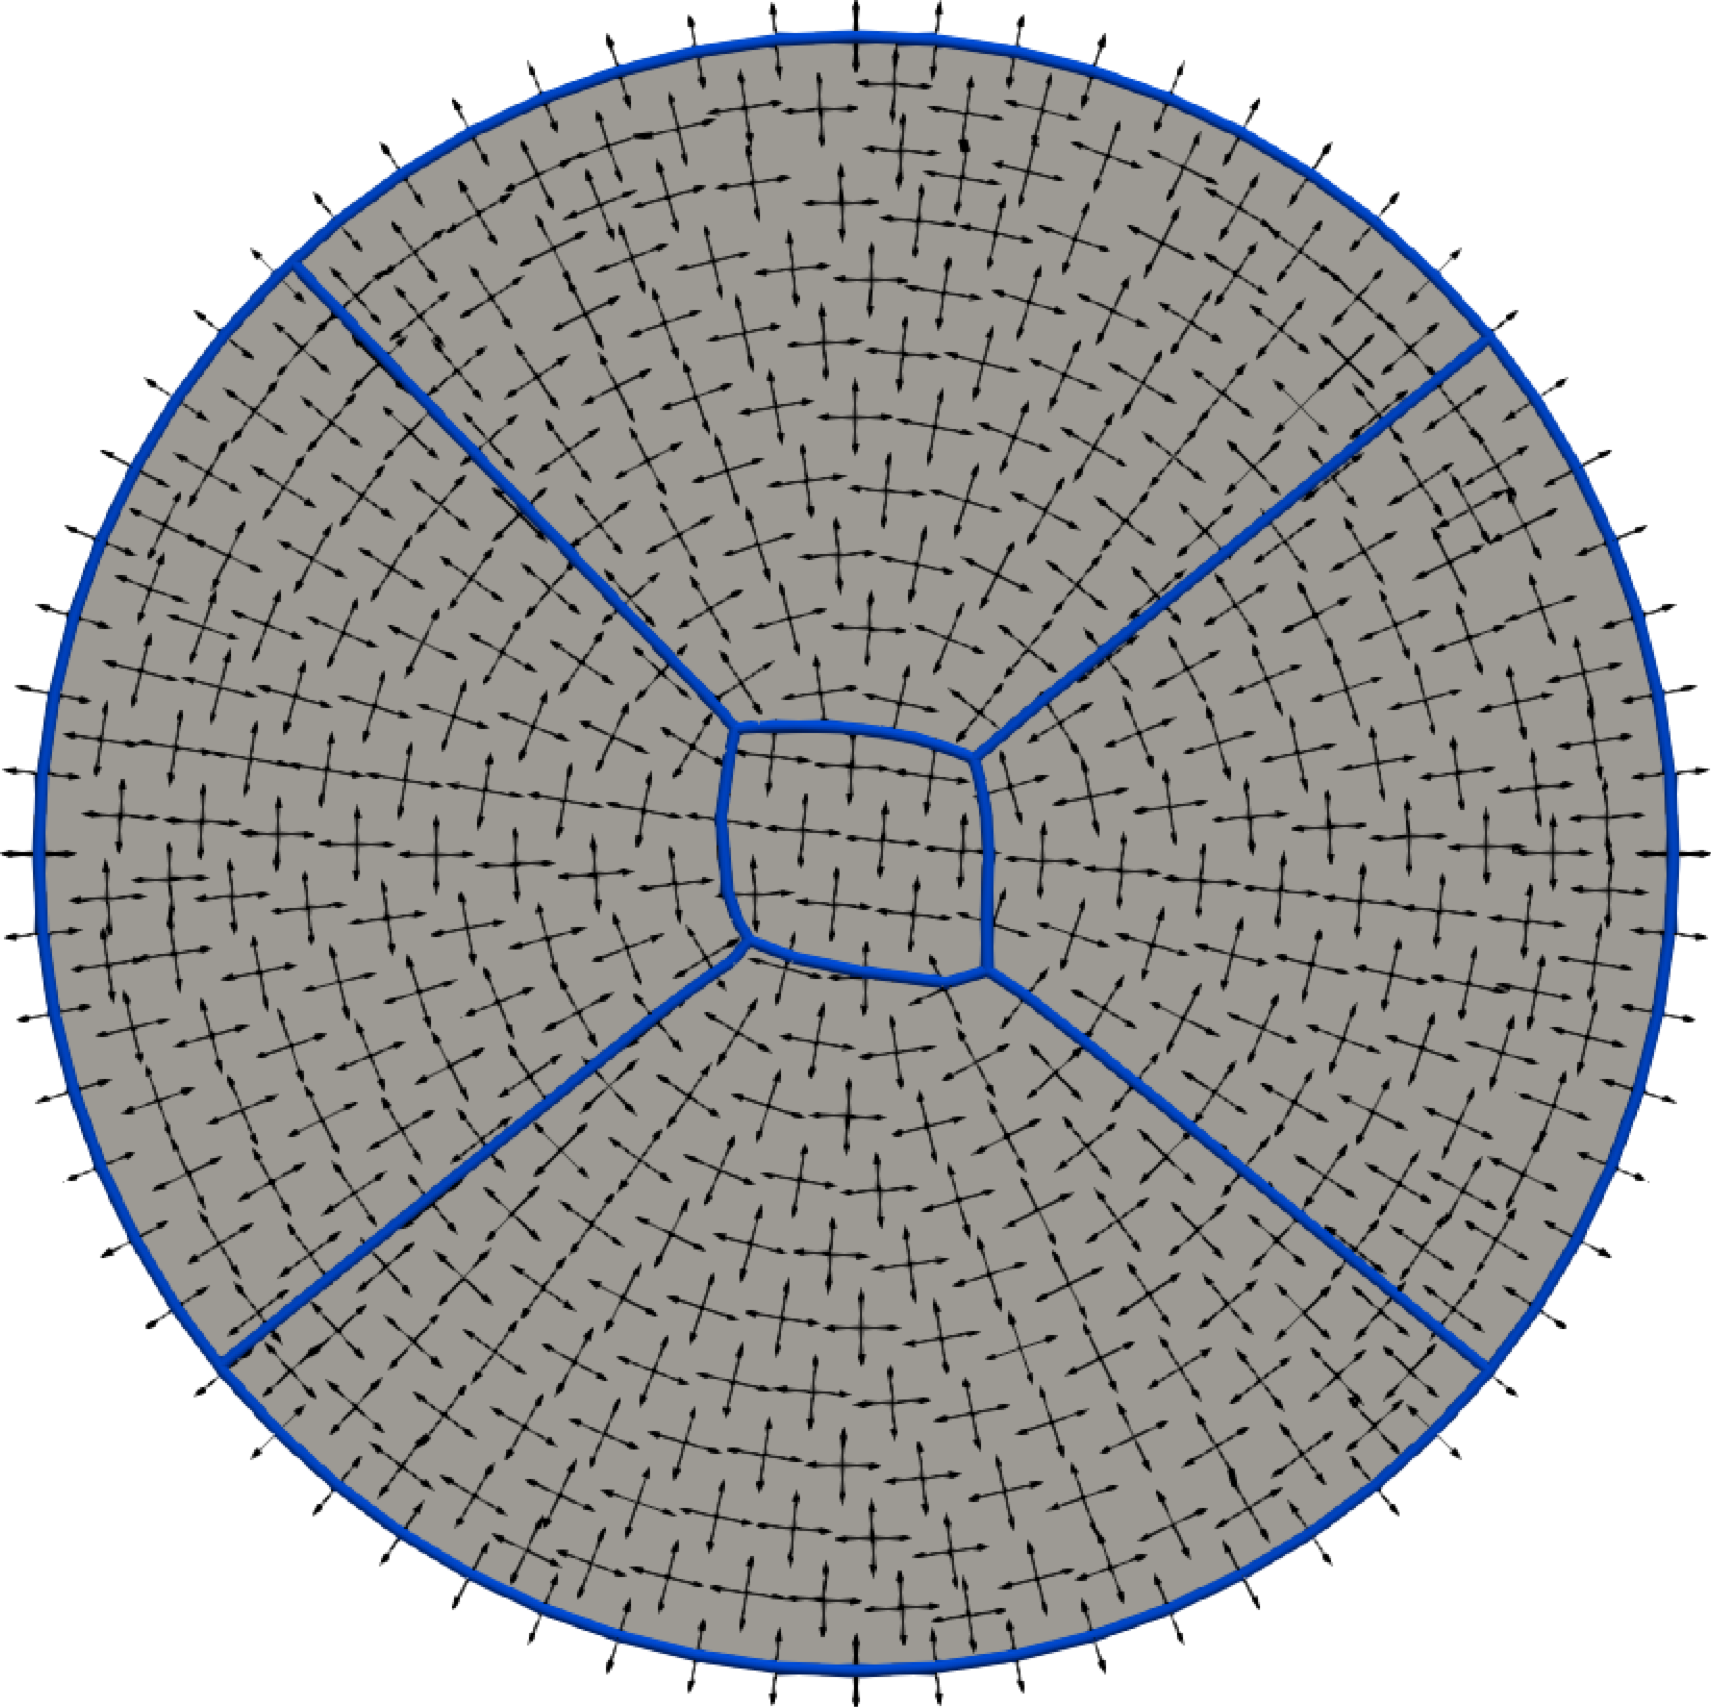
\includegraphics[scale=0.27]{images/explosion_1.pdf}
\hfill
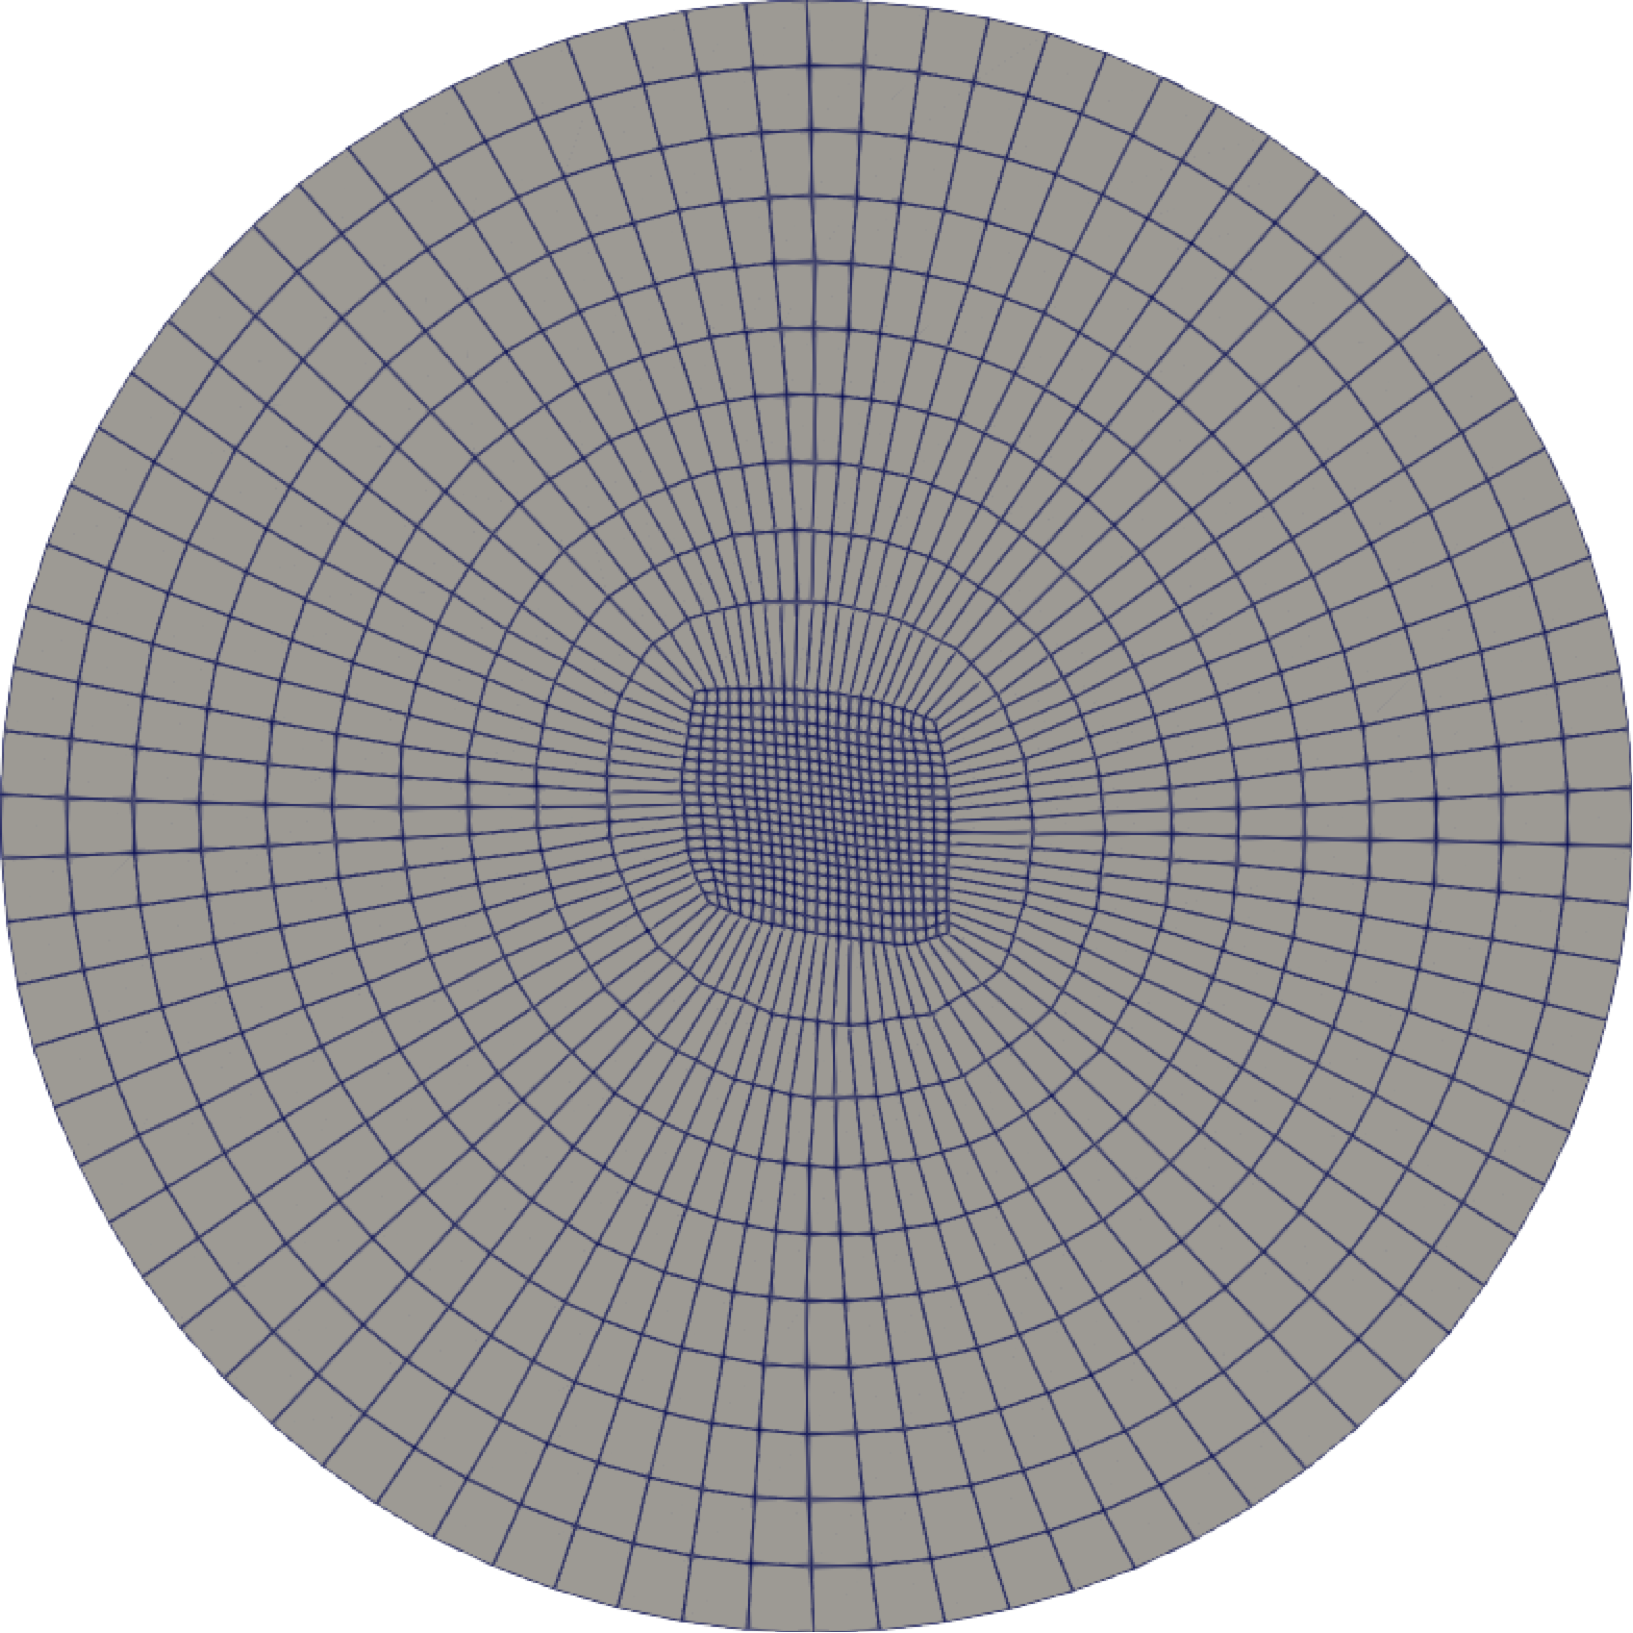
\includegraphics[scale=0.27]{images/explosion_2.pdf}
\caption{Première itération.}
\label{fig:iteration_1}
\end{figure}

\begin{figure}[h!]
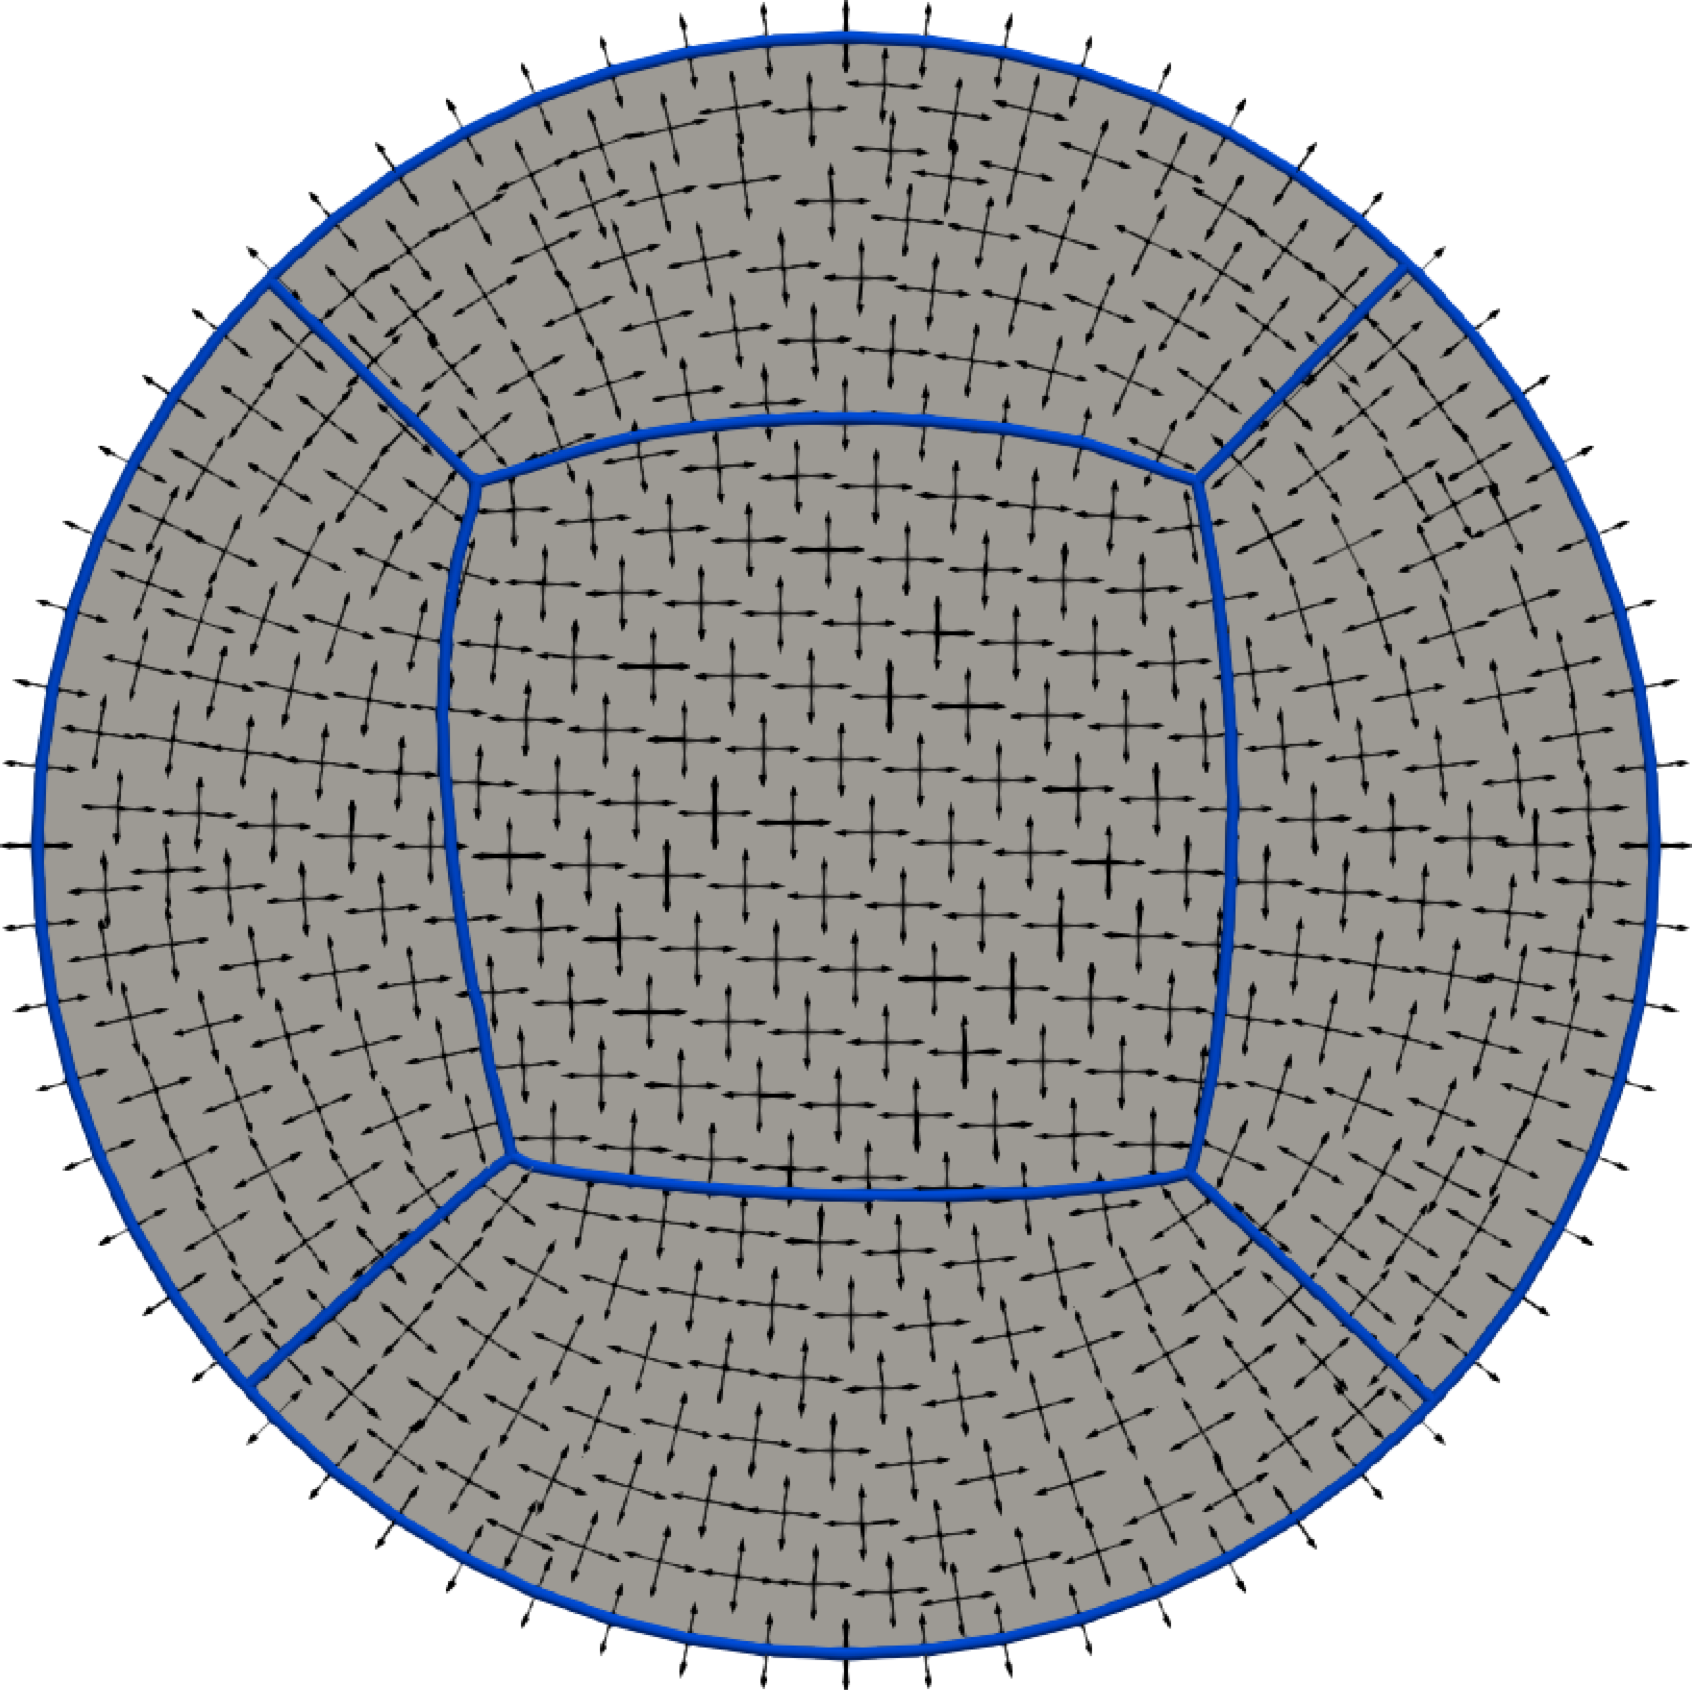
\includegraphics[scale=0.27]{images/explosion_3.pdf}
\hfill
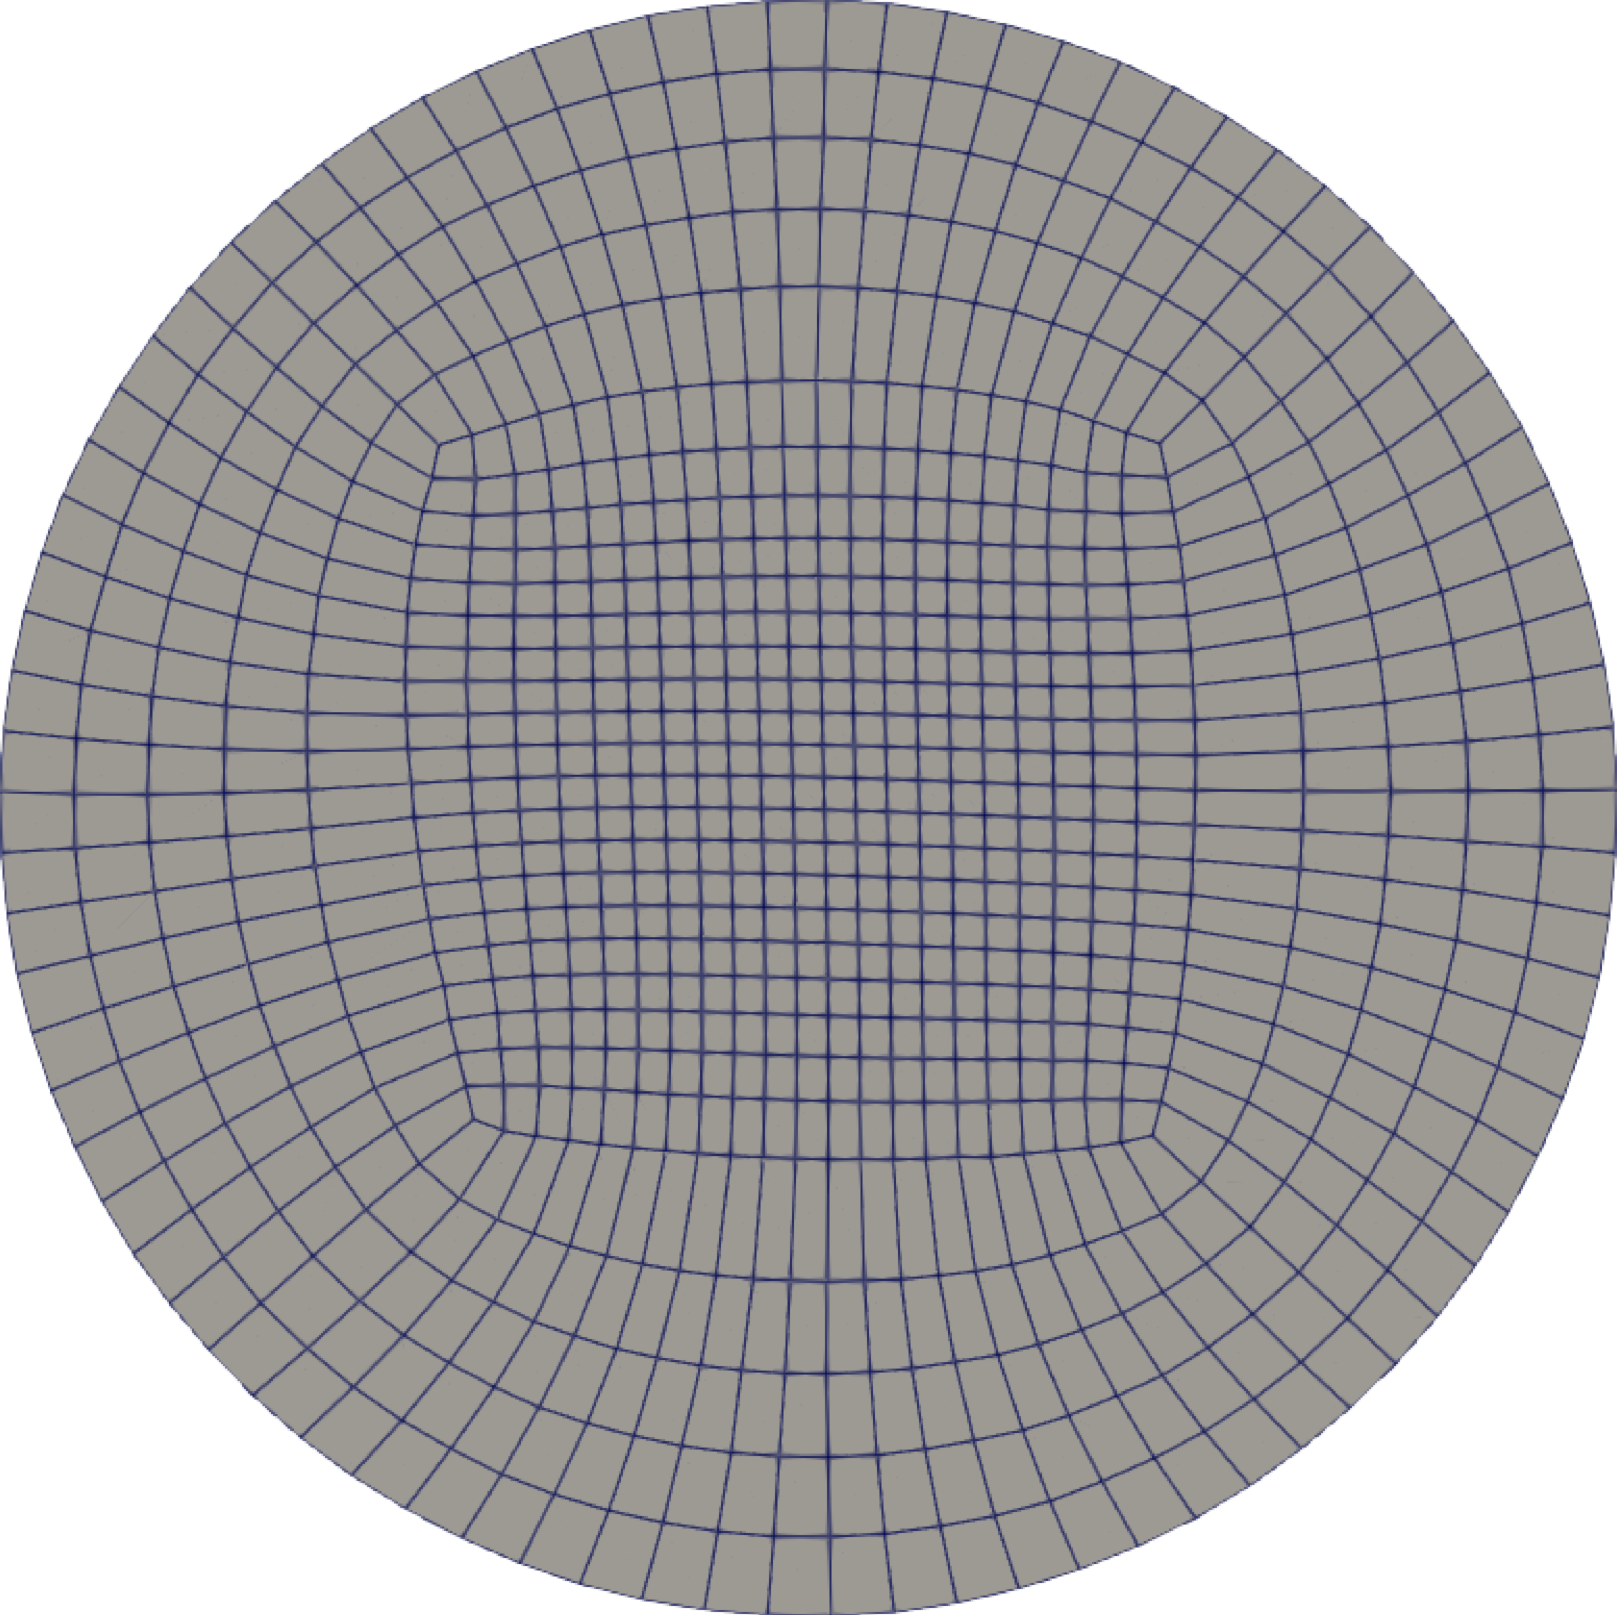
\includegraphics[scale=0.27]{images/explosion_4.pdf}
\caption{Deuxième itération.}
\label{fig:iteration_2}
\end{figure}

Dans cet exemple particulier, nous commençons par générer un maillage en utilisant un champ de croix dérivé de la résolution de l'équation de Laplace, comme illustré dans la figure \ref{fig:iteration_1}. Ensuite, nous identifions un point dans le domaine où la densité de maille semble plus élevée, et nous itérons le calcul du champ de croix en utilisant la même équation. Cependant, cette fois, dans les conditions aux limites, nous attribuons une croix arbitraire au point spécifié. Le résultat de cette itération est le champ de croix présenté dans la figure \ref{fig:iteration_2}, qui est ensuite utilisé pour générer le maillage illustré sur la même figure. On peut observer que les points singuliers s'éloignent les uns des autres, permettant ainsi d'obtenir des partitions plus homogènes. Ce processus itératif peut être poursuivi en identifiant d'autres points dans le domaine où la densité de maille est élevée, puis en répétant l'opération décrite précédemment.\\\\
Une autre approche envisageable consiste à rechercher des points d'équilibre, où ces points sont relativement équidistants les uns des autres ainsi que des bords du domaine. En utilisant ensuite la méthode présentée dans la sous-section \ref{subsec:laplace_equation_generation}, nous générons un champ de croix sur le domaine que nous alignons ensuite sur le bord du domaine à partir de l'opération d'alignement. Une hypothèse sous-jacente est que, en garantissant une distance équidistante des points d'équilibre par rapport aux bords, le champ de croix résultant pourrait présenter des points singuliers plus uniformément répartis. Cette uniformité pourrait contribuer à obtenir un partitionnement avec des partitions plus homogènes. Pour identifier ces points d'équilibre, une approche pourrait consister, dans un premier temps, à déterminer la distance moyenne entre le bord et l'intérieur du domaine. On peut mettre en œuvre cette approche en attribuant des valeurs décroissantes aux triangles du bord vers l'intérieur du domaine, simulant ainsi une progression de front. En identifiant ensuite les sommets correspondants à la valeur moyenne des attributions des triangles, on sélectionne parmi ces sommets ceux qui sont le plus équidistants possible. Comme illustré sur la figure \ref{fig:coloriage}, un coloriage des triangles du bord vers l'intérieur du domaine permet de délimiter des zones d'équilibre, où l'on pourrait positionner les points singuliers sur la frontière.\\\\
\begin{figure}[h!]
\centering
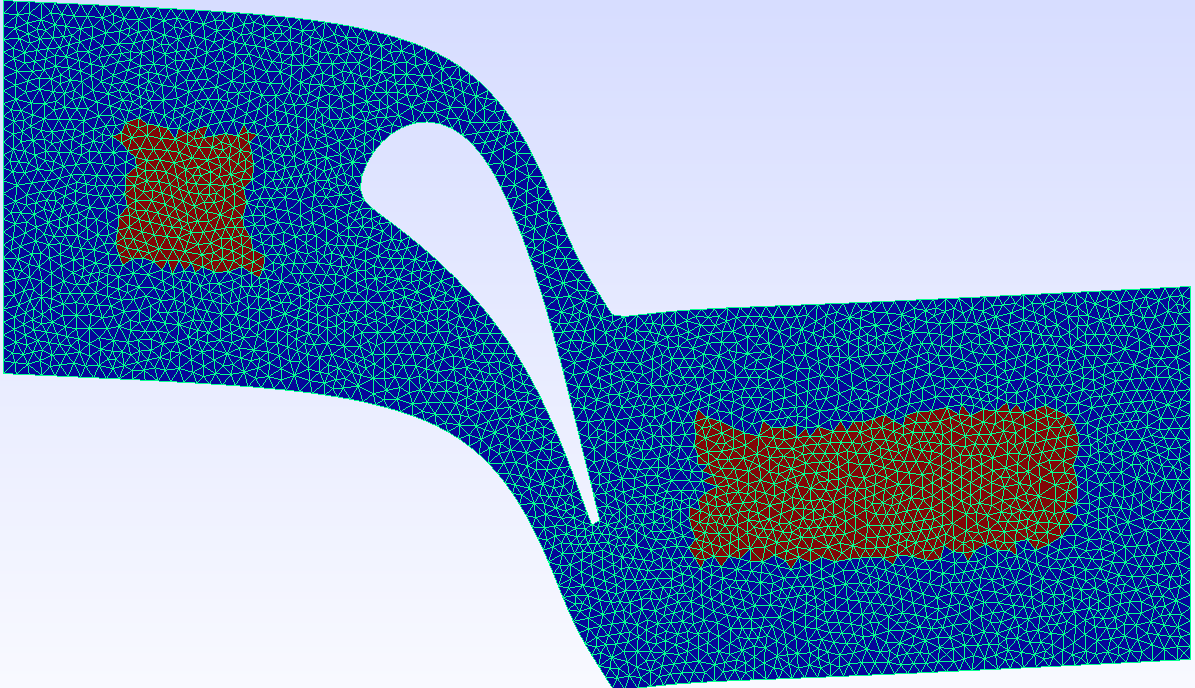
\includegraphics[scale=0.35]{images/coloriage.png}
\caption{Détection de zones d'équilibres.}
\label{fig:coloriage}
\end{figure}
Ces deux approches, telles qu'elles sont exposées, présentent une limitation majeure, à savoir qu'elles ne permettent pas de contrôler la répartition des séparatrices dans le domaine une fois que les points singuliers sont disposés de manière équidistante les uns par rapport aux autres. La question qui se pose est donc de savoir s'il est possible d'influencer le champ de manière à, par exemple, maintenir la connectivité des séparatrices au cours des itérations successives dans le premier cas.


\subsection*{Comment adapter le maillage?}

L'adaptation du maillage à un contexte physique donné représente également une problématique centrale dans les simulations numériques. Les approches de génération explorées dans cette thèse ont pour objectif de converger vers cette application. En effet, l'idée de choisir un champ de croix et de le modifier pour qu'il serve à mailler un domaine découle du souhait de conserver le plus de caractéristiques possible dans le champ initial, garantissant ainsi que le maillage généré soit adapté au contexte d'où a été récupéré ce champ. Ce champ initial peut être déduit d'une estimation à posteriori.

Dans ce sens, une piste consiste à proposer un champ de croix aligné le plus possible sur une référence ($C_r$, d'angle $\theta$) et respectant des contraintes issues d'un autre champ de croix ($C_a$, d'angle $\phi$), typiquement garder le plus de caractéristiques possibles d'une estimation a posteriori et assurer l'alignement avec le bord du domaine. On cherche donc à résoudre le système:
\begin{equation}
\begin{cases}
    \tilde{\theta} := \theta + \alpha\phi \in C^1(\Omega), \\\\
    \min_{\substack{\alpha=1 \\ \partial\Omega}} \left\lvert \theta - \tilde{\theta} \right\rvert,
\end{cases}
\end{equation}
ce qui revient à résoudre au sens champ de croix (possibilité de $+k\pi/2$ sur les angles):
$$
\alpha^* = \arg\min_{\alpha\in C^1(\Omega,[0,1]), \alpha=1 \text{ sur } \partial\Omega} \left( \lVert \alpha\phi \rVert_\infty + \lambda \lVert \nabla (\alpha\phi) \rVert_\infty \right).
$$
En éléments finis $\mathbb{P}_1$, on a:
\begin{equation}
\begin{aligned}
    \lVert \alpha\phi \rVert_{L^\infty(T)} &= \max_{S \text{ sommets de } T} \left( \min_{k\in[-4,3]} \left\lvert \alpha(S)\phi(S) + k\pi/2 \right\rvert \right), \\\\
    \lVert \nabla (\alpha\phi) \rVert_{L^\infty(T)} &= \min_{k\in[0,3]^3} \left\lVert \sum_{i=1}^{3} \frac{\alpha(S_i)\phi(S_i) + k_i\pi/2}{h_{T,i}} \right\rVert,
\end{aligned}
\end{equation}
où $h_{T,i}$ est la longueur de la hauteur du triangle $T$ issue du sommet $S_i$ et $h_{T,i}$ la hauteur normalisée. Ainsi,
\[
\begin{array}{lcl}
\lVert \alpha\phi \rVert_{C^1(\Omega)} &=& \max_{S \text{ sommets de } T (\Omega)} \left( \min_{k\in[0,3]} \left\lvert \alpha(S)\phi(S) + k\pi/2 \right\rvert \right)\\\\
&&+ \lambda \max_{T\in\mathcal{T}(\Omega)} \left( \min_{k\in[0,3]^3} \left\lVert \sum_{i=1}^{3} \frac{\alpha(S_i)\phi(S_i) + k_i\pi/2}{h_{T,i}} \right\rVert \right).
\end{array}
\]
Cette approche cependant ne marche pas avec les angles représenté en $\mathbb{P}_1$. L'alternative consiste à trouver $\alpha \in C^1(\Omega)$ tel que:
\begin{equation}
\begin{cases}
    \tilde{\theta} := \theta + \alpha \in C^1(\Omega), \\\\
    \min \left\lvert \theta - \tilde{\theta} \right\rvert, \\\\
    \alpha = \phi - \theta \text{ sur } \partial\Omega.
\end{cases}
\label{eqn:adapt_eqn_1}
\end{equation}
En pratique, on va chercher $\alpha_h \in\mathbb{P}_1(\Omega)$ qui approche $\alpha$. Le contrôle $C^1$ de la solution n'est pas possible à rendre si on peut toujours supposer que $\alpha_h$ est une approximation nodale d'une fonction $\alpha$ plus régulière. En particulier, cette considération peut s'appliquer sur les nœuds d'un triangle donné en faisant par exemple passer $\alpha_h$ de 1 à 0 brutalement sur un/deux nœud/s du triangle, ce qui revient à dire que $\lVert \nabla\alpha \rVert \leq h^{-1}$ où $h$ est la hauteur du triangle dans le sens de variation considéré. Il s'en suivrait alors de trop rapides variations de la fonction $\tilde{\theta}$ reconstruite (et ses lignes de champs varieraient très vite ce qui engendrerait des éléments très déformés et/ou très petits). Pour pallier ce problème, on impose une variation maximale à ne pas dépasser notée $\nu > 0$.

De plus, dans le cadre du maillage quadrilatéral, si $\theta$ représente l’angle du champ de croix aligné avec le bord, alors, pour un domaine n’étant pas à 4 côtés, on sait que $\theta$ présentera des singularités dans le domaine et donc ne sera pas $C^1(\Omega)$. Le système \eqref{eqn:adapt_eqn_1} n’a donc pas de solution. Toutefois, si $\theta$ est aligné avec le bord alors il va exister un voisinage $V$ de $\partial\Omega$ privé de $\partial\Omega$ dans lequel $\theta$ sera $C^1$. On peut alors essayer de résoudre \eqref{eqn:adapt_eqn_1} pour un $\alpha$ à support dans $V$ et $C^1$, $\tilde{\theta}$ sera alors l’angle du champ de croix obtenu par $R(\alpha)C_r$, qui sera un champ de croix presque-$C^1$ et de singularités coïncidentes avec celles de $C_r$.

En outre, pour une question d’efficacité nous allons remplacer la résolution du problème d’optimisation globale \eqref{eqn:adapt_eqn_1} en une série d’optimisations locales. L’idée est de procéder triangle par triangle en notant que la contrainte de bord permet de définir explicitement la valeur de $\alpha$. La formulation éléments finis de \eqref{eqn:adapt_eqn_1} avec cette contrainte revient à trouver $\alpha_h\in\mathbb{P}_1(\Omega)$ tel que:
\begin{equation}
\begin{cases}
\tilde{\theta}_h := \theta_h + \alpha_h \in P^1(\Omega), \\\\
\min \left|\theta_h - \tilde{\theta}_h\right|, \\\\
\alpha_h = \phi_h - \theta_h, \ \partial\Omega, \\\\
\text{Supp}\,\alpha_h \subset V, \\\\
\|\nabla\alpha_h\| \leq \nu.
\end{cases}
\label{eqn:adapt_eqn_2}
\end{equation}
En pratique, la résolution de \eqref{eqn:adapt_eqn_2} peut être effectuée via la construction locale de $\tilde{\theta}_h$ sur chaque triangle $T\in\mathcal{T}_h$ suivante:\\
\begin{enumerate}
    \item Affectation des valeurs $\tilde{\theta}_h(S) = \phi_h(S)$ pour tous les nœuds $S \in \partial\Omega$,\\
    \item Tant qu'il reste des triangles à traiter :\\
    \begin{enumerate}
        \item Suppression des triangles ayant déjà $\tilde{\theta}_h$ calculé sur les 3 nœuds de la liste des triangles à traiter,\\
        \item Recherche des triangles $T$ pour lesquels $\tilde{\theta}_h$ est définie pour 2 nœuds sur 3,\\
        \item Si les valeurs de $\tilde{\theta}_h$ pour 2 nœuds sur 3 de $T$ sont nulles alors $T$ est retiré de la liste à évaluer,\\
        \item Sur $T_h$ on note $S_1$ et $S_2$ les nœuds pour lesquels $\tilde{\theta}_h$ a été évaluée, $S_3$ le troisième sommet, $\overrightarrow{h_3}$ la hauteur normalisée issue de $S_3$, $X_h = x_hS_2 +(1-x_h)S_1$ le pied de la hauteur et $h_3 = |X_h - S_3|$,\\
        \item À partir d'une valeur $\tilde{\theta}_h(S_1) \left[ \frac{\pi}{2} \right]$, on calcule
        \[
        \tilde{\theta}_h(S_2, S_1) := \arg\min_{y\in{\tilde{\theta}_h(S_2)+k\pi/2, k\in\mathbb{Z}}}
        \left|y - \tilde{\theta}_h(S_1)\right|,
        \]
        et on note $\beta = x_h \tilde{\theta}(S_2, S_1) + (1 - x_h)\tilde{\theta}(S_1)$,\\
        \item Calcul des variations maximales possibles pour $\theta \in [\theta^-, \theta^+]$ :
        \[
        \theta^\pm = \beta \pm |h_3|\nu\overrightarrow{h_3}.
        \]
        \item La solution est alors simplement obtenue par
    \[
    \tilde{\theta}_h(S_3) = \min(\theta^+, \max(\theta^-, \theta_h(S_3))),
    \]
    et le triangle est marqué comme traité.
    \end{enumerate}
\end{enumerate}
La fonction $\alpha_h = \tilde{\theta}_h - \theta_h$ vérifie alors les propriétés attendues dans \eqref{eqn:adapt_eqn_2}. Concernant le choix de $\nu$, on prend typiquement
\[
\nu = \frac{\pi}{4d} \mbox{ avec } d = nh,
\]
où $h$ est une grandeur caractéristique du maillage (typiquement la hauteur minimale) et $n > 0$. Cela porte le support de $\alpha_h$ typiquement à $d$ de $\partial\Omega$. Le $\pi/4$ représente la valeur maximale de variation attendue sur les angles, vu qu’ils sont définis par modulo $\pi/2$.\\\\
Une autre vision pour l'adaptation de maillage serait d'utiliser la méthode d'optimisation CVT en tenant compte d'une densité d'erreur à postéririori permettant d'influer le deplacement des noeuds. Une telle approche cependant en opposition avec ce qui a été présenté plus haut adapte directement le maillage quadrilatéral générer au lieu d'adapté le champ de croix dont il est issu. On conserve la nature en structure par bloc du maillage ainsi que les connectivités.

\subsection*{Comment gérer les cycles limites ?}
Un défi crucial associé à la méthode de génération de maillage quadrilatéral à partir de champs de croix réside dans la gestion des cycles limites. En effet, le contrôle sur la trajectoire des séparatrices n'est pas a priori déterminé, ce qui conduit souvent à un échec du partitionnement en présence de cycles limites, surtout dans le cas des surfaces courbes dans l'espace. Nous proposons ici une approche de solution pour ce problème. L'idée principale consiste à arrêter l'intégration des séparatrices convergentes en cycle lorsque celles-ci interagissent avec une autre séparatrice. À la fin du processus de partitionnement, on se retrouve avec des blocs n'ayant pas nécessairement quatre côtés.

Une première approche suggère d'utiliser une subdivision de Catmull-Clark pour subdiviser tous les blocs en des régions à quatre côtés tout en préservant la conformité entre les blocs. Cependant, cette méthode peut potentiellement générer des nœuds très irréguliers avec des valences élevées. Une autre piste, basée sur cette dernière approche, consiste à repérer les blocs qui ne sont pas à quatre côtés et à les subdiviser de manière spécifique. Supposons que toutes les partitions obtenues après le partitionnement ont au moins trois sommets. Lorsque le nombre de sommets est strictement supérieur à 4, on identifie quatre nœuds que l'on considère comme les coins du bloc. Ensuite, on associe deux à deux les sommets appartenant aux côtés non adjacents et les sommets appartenant aux côtés adjacents en utilisant un nœud singulier. À ce stade, on obtient une région qui a des sommets supplémentaires (autres que les coins choisis) uniquement sur un côté. On peut utiliser la subdivision de Catmull-Clark à cette étape. L'avantage de cette approche est la réduction du nombre de blocs à créer avec la subdivision de Catmull-Clark, diminuant ainsi la valence des points irréguliers générés. Pour les partitions de 3 et 5 côtés, on procède directement à la subdivision de Catmull-Clark. Ensuite, il est nécessaire de gérer la fusion des séparatrices d'un bloc à l'autre afin de ne pas engendrer de nouveaux cycles limites. Il est important de noter que les blocs générés avec une telle approche seront potentiellement très déformés. Cet artefact peut être résolu en optimisant le maillage généré via la méthode CVT présentée dans la section \ref{sec:Homogeneisation_algo}. Nous illustrons les différents cas de décompositions sur les figures \ref{fig:cycle_1}, \ref{fig:cycle_2} et \ref{fig:cycle_3}. Les points noirs sur les bord représentent les points d'arêts des lignes de champ convergeant en cycle limite.


\begin{figure}[h!]
\centering
\begin{subfigure}{0.49\textwidth}
    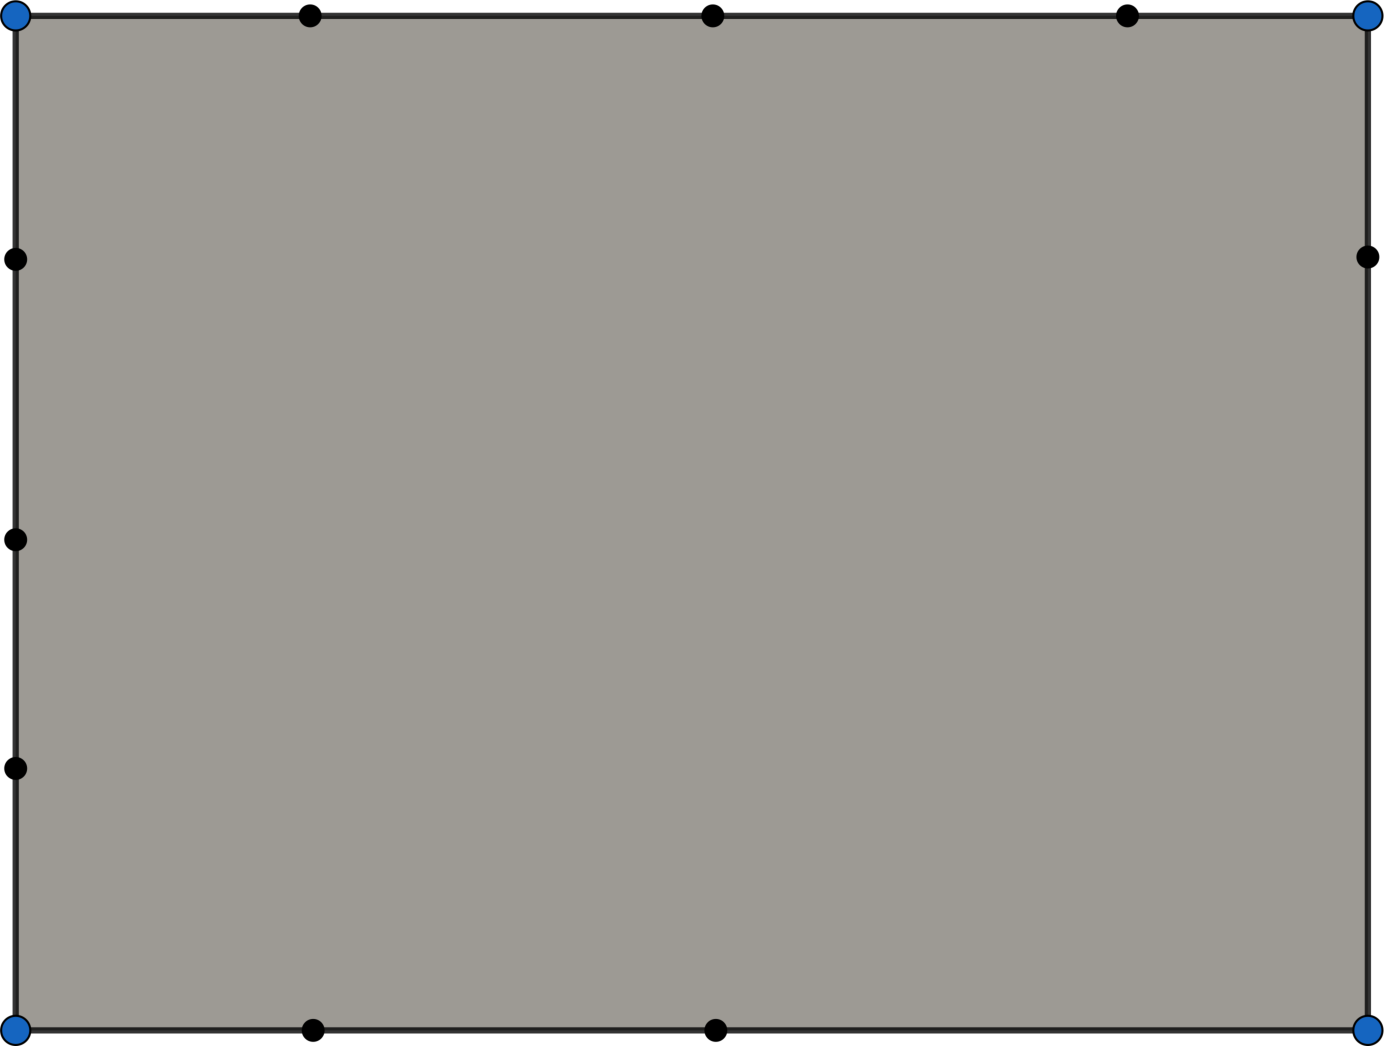
\includegraphics[width=\textwidth]{images/limit_cycle_1.pdf}
    %\caption{Champ scalaire $\phi_h$ (en randian)}
    %\label{fig:alignment_2}
\end{subfigure}
\hfill
\begin{subfigure}{0.49\textwidth}
    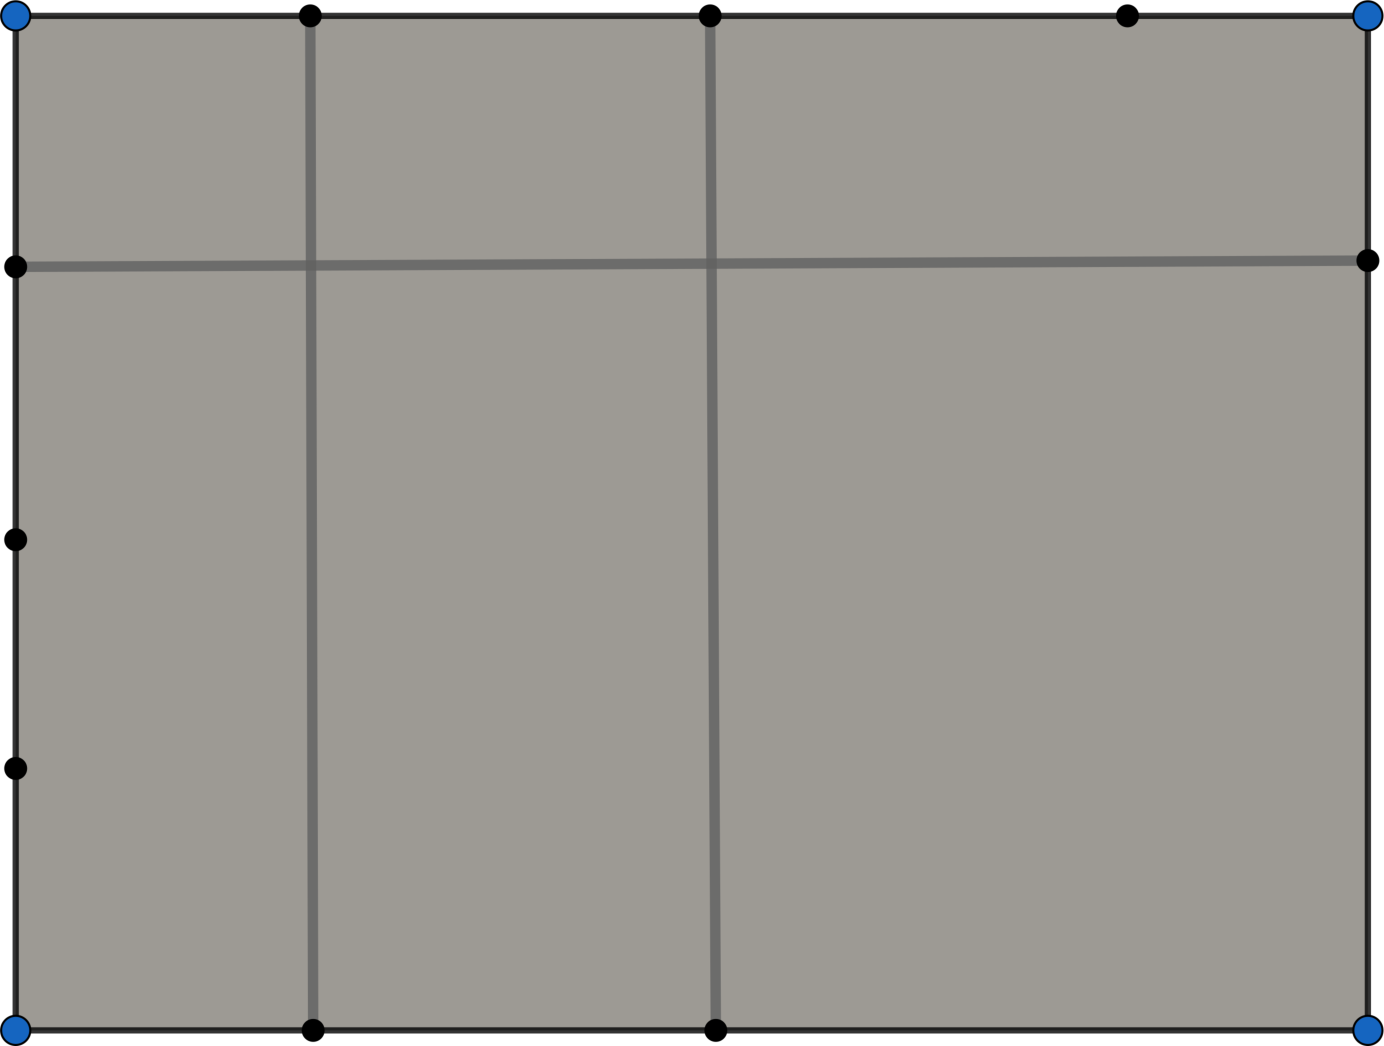
\includegraphics[width=\textwidth]{images/limit_cycle_2.pdf}
    %\caption{Maillage.}
    %\label{fig:alignment_4}
\end{subfigure}
\caption{Premier cas.}
\label{fig:cycle_1}
\end{figure}


\begin{figure}[h!]
\centering
\begin{subfigure}{0.49\textwidth}
    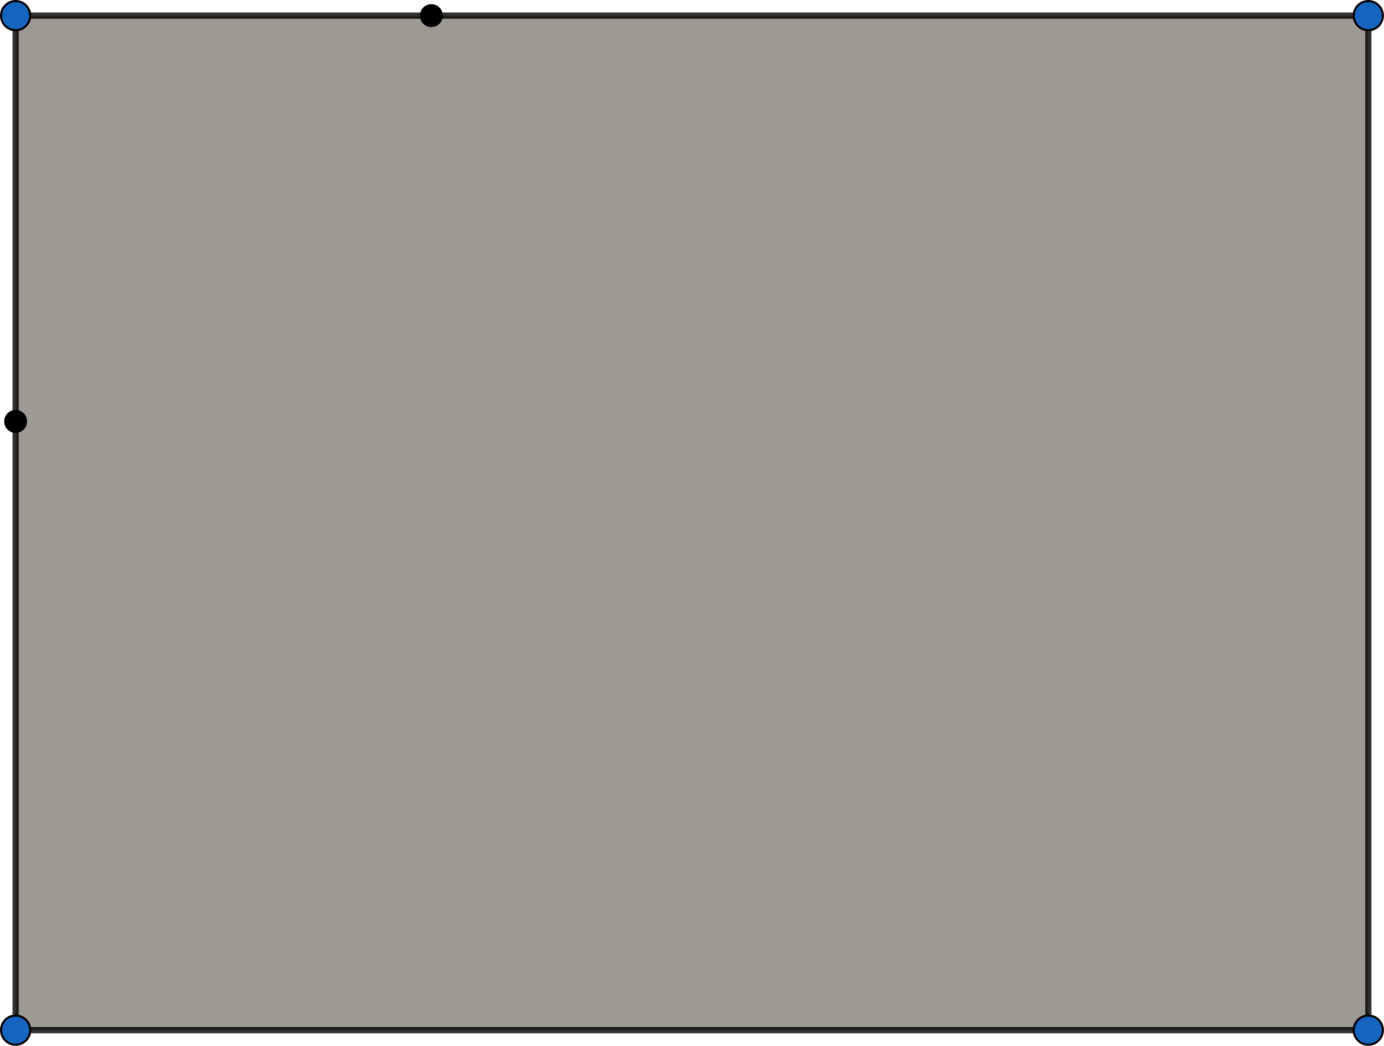
\includegraphics[width=\textwidth]{images/limit_cycle_3.pdf}
    %\caption{Champ scalaire $\phi_h$ (en randian)}
    %\label{fig:alignment_2}
\end{subfigure}
\hfill
\begin{subfigure}{0.49\textwidth}
    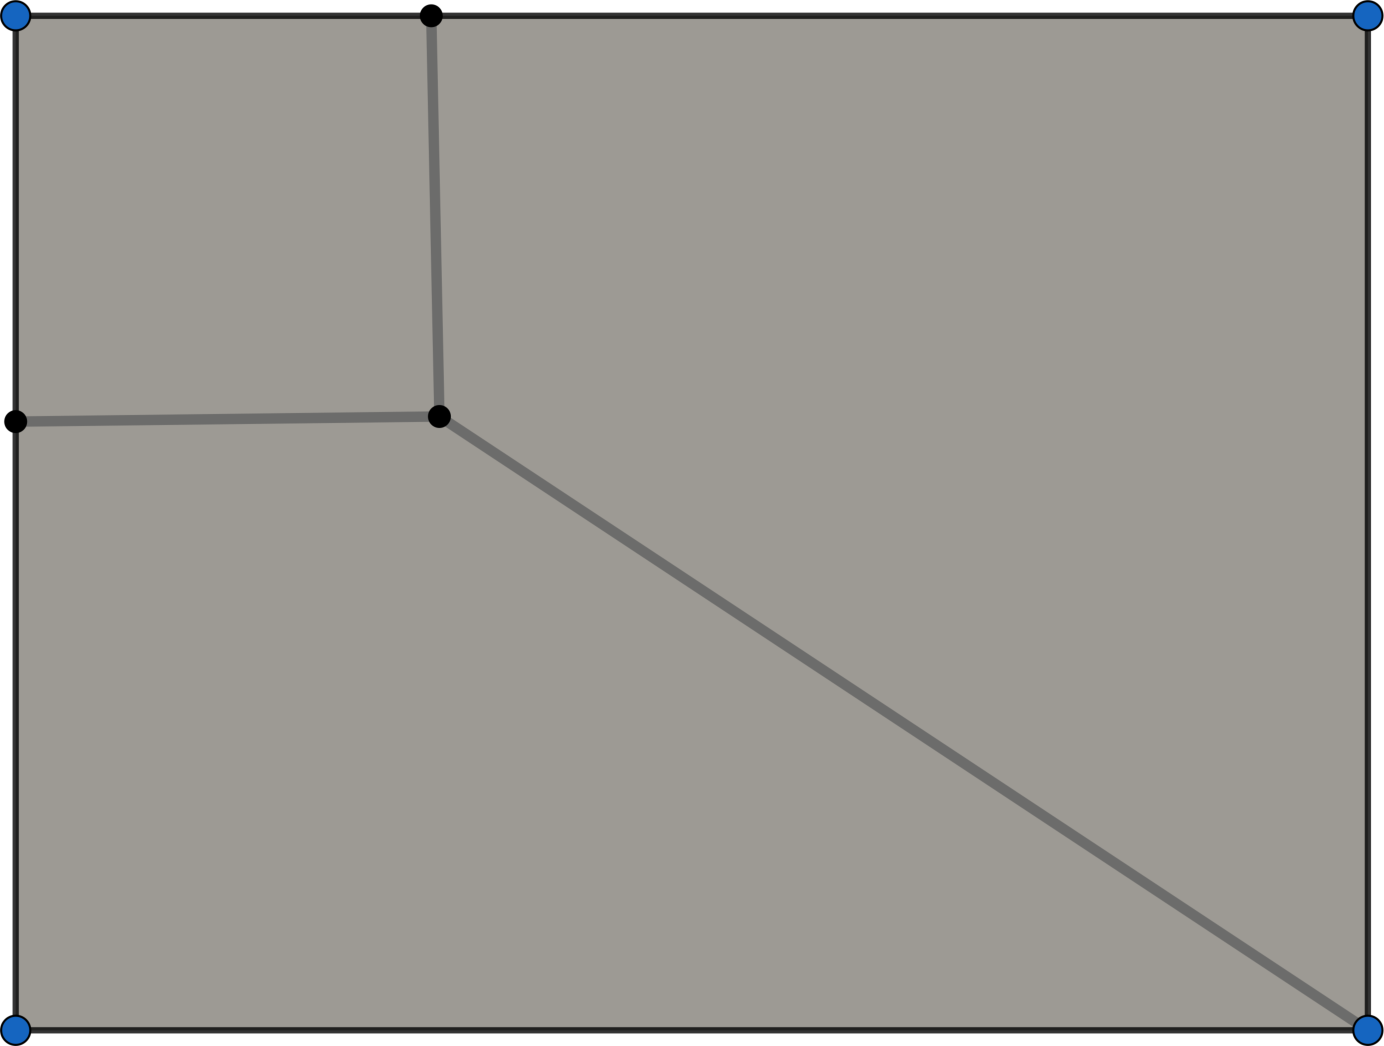
\includegraphics[width=\textwidth]{images/limit_cycle_4.pdf}
    %\caption{Maillage.}
    %\label{fig:alignment_4}
\end{subfigure}
\caption{Deuxième cas.}
\label{fig:cycle_2}
\end{figure}


\begin{figure}[h!]
\centering
\begin{subfigure}{0.49\textwidth}
    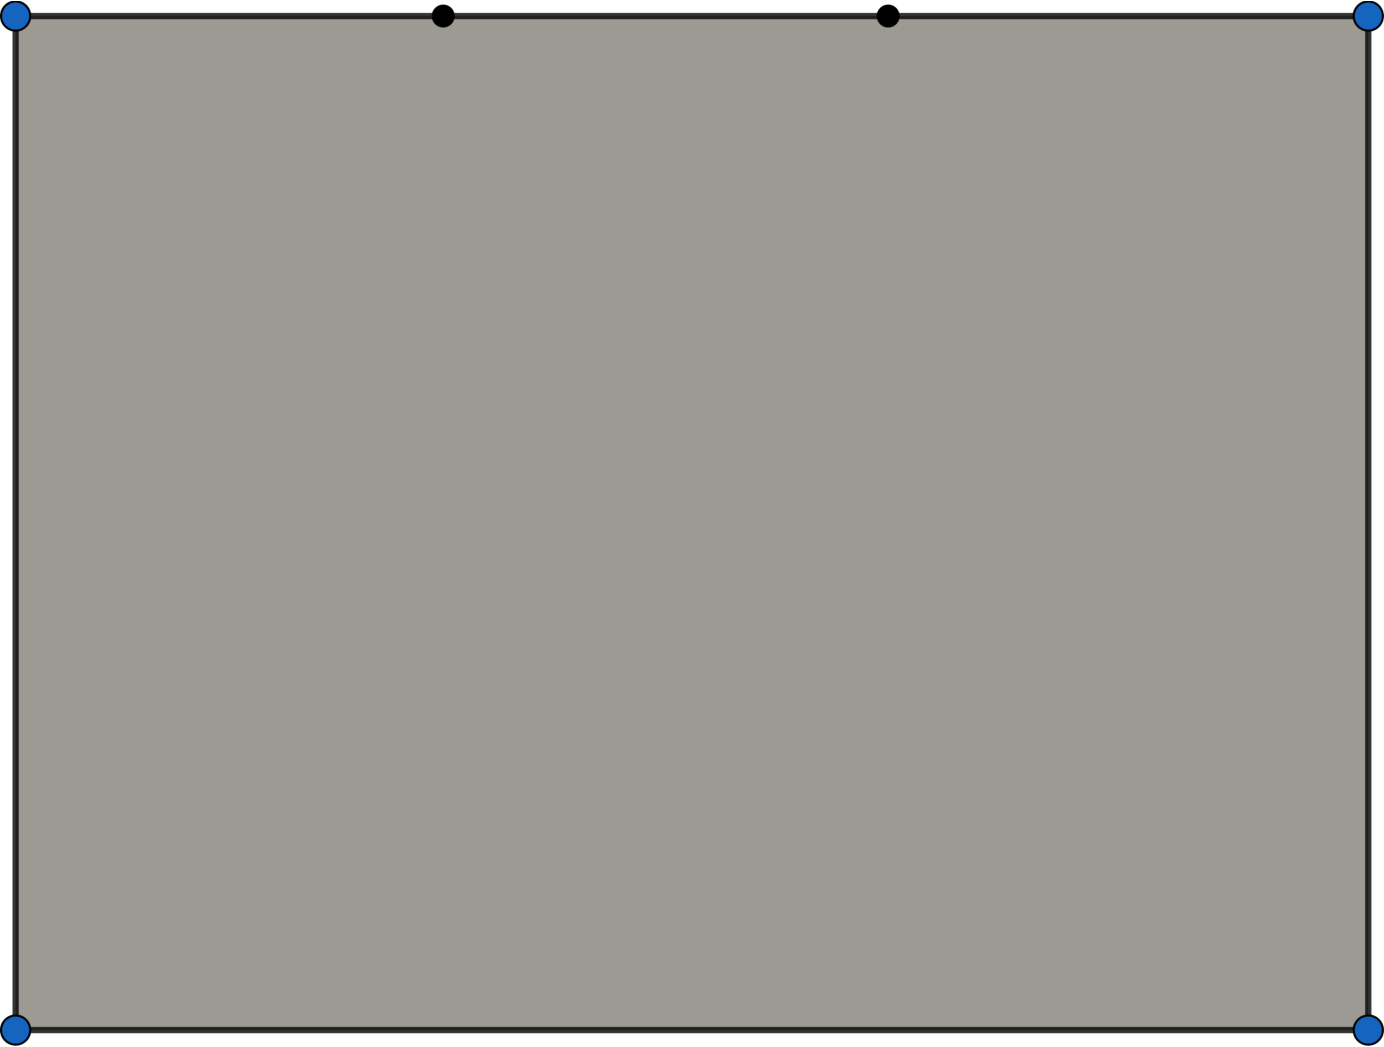
\includegraphics[width=\textwidth]{images/limit_cycle_5.pdf}
    %\caption{Champ scalaire $\phi_h$ (en randian)}
    %\label{fig:alignment_2}
\end{subfigure}
\hfill
\begin{subfigure}{0.49\textwidth}
    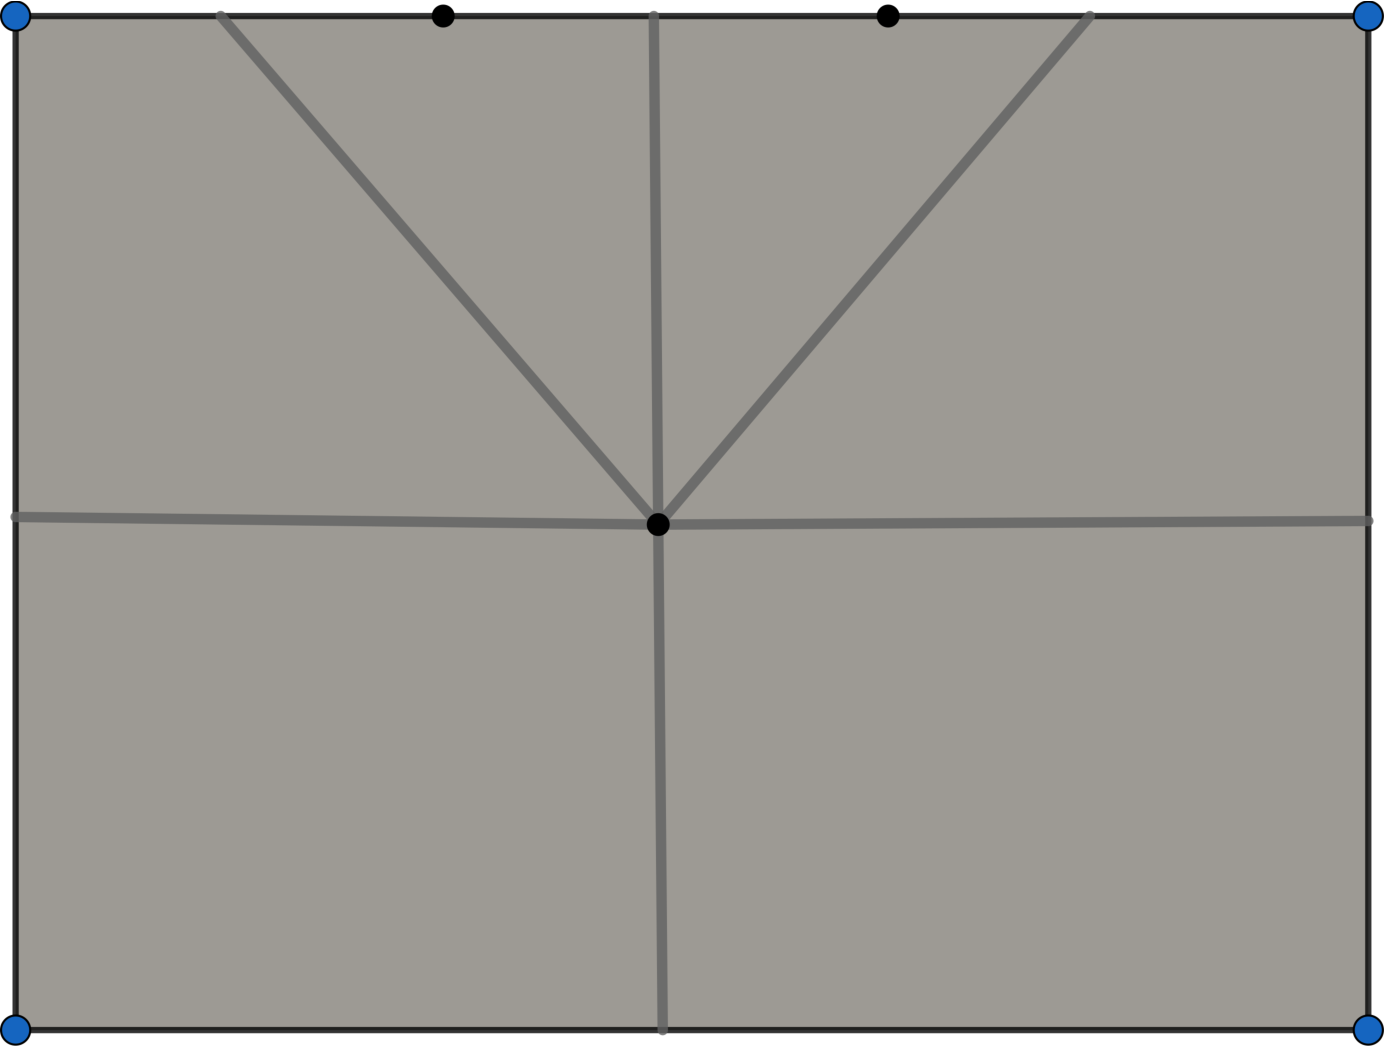
\includegraphics[width=\textwidth]{images/limit_cycle_6.pdf}
    %\caption{Maillage.}
    %\label{fig:alignment_4}
\end{subfigure}
\caption{Troisième cas.}
\label{fig:cycle_3}
\end{figure}


\subsection*{Face à un domaine périodique}

Une autre considération importante concerne la gestion des domaines périodiques, c'est-à-dire les domaines où les conditions aux bords sont périodiques d'un bord à un autre. C'est notamment le cas du modèle LS89, détaillé dans \cite{gourdain2010advanced}, où, par exemple, le bord supérieur et le bord inférieur doivent être connectés par des conditions aux bords périodiques. La question qui se pose est donc de savoir comment construire un maillage structuré par bloc avec la méthode des champs de croix de manière à générer des blocs conformes périodiquement d'un bord à l'autre. Sur la figure \ref{LS89_transparent} où nous avons superposé le maillage en bloc structuré du LS89, on observe que les blocs ne sont pas conformes périodiquement, ce qui pose problème pour l'exploitation de la nature structurée en bloc dans un contexte périodique.

\begin{figure}[!h]
\centering
\includegraphics[scale=0.5]{images/LS89_transparent.png}
\caption{Superposition du maillage du LS89.}
\label{LS89_transparent}
\end{figure}


\subsection*{Mailles d'ordre supérieur}

Dans notre étude, les quadrilatères construits le long du bord du domaine ont leurs nœuds positionnés le long des arêtes du maillage triangulaire utilisé pour la construction. Cependant, dans les codes de calcul, il peut être nécessaire d'interpoler la courbure le long de la frontière du maillage quadrilatéral, surtout dans le cas de conditions limites impliquant la dérivée normale, telles que les conditions aux limites de Neumann et de Robin. Face à une telle situation, les calculs de reconstitution de la normale dépendront de la résolution obtenue pour les mailles du bord lors de la construction du maillage quadrilatéral (voir la figure \ref{fig:mail_tri_vs_mail_quad}). Ainsi, si la finesse demandée pour le maillage quadrilatéral est supérieure à celle du maillage triangulaire servant de base à la construction, il sera impossible de récupérer de manière précise les informations avec les nœuds de bord du maillage quadrilatéral. Par conséquent, la définition explicite de $\Omega_{\tilde{h}}$ permet de se libérer des triangles de bord et de ne plus être contraint par cette dépendance.\\\\
\begin{figure}[h!]
\centering
\begin{subfigure}{0.6\textwidth}
    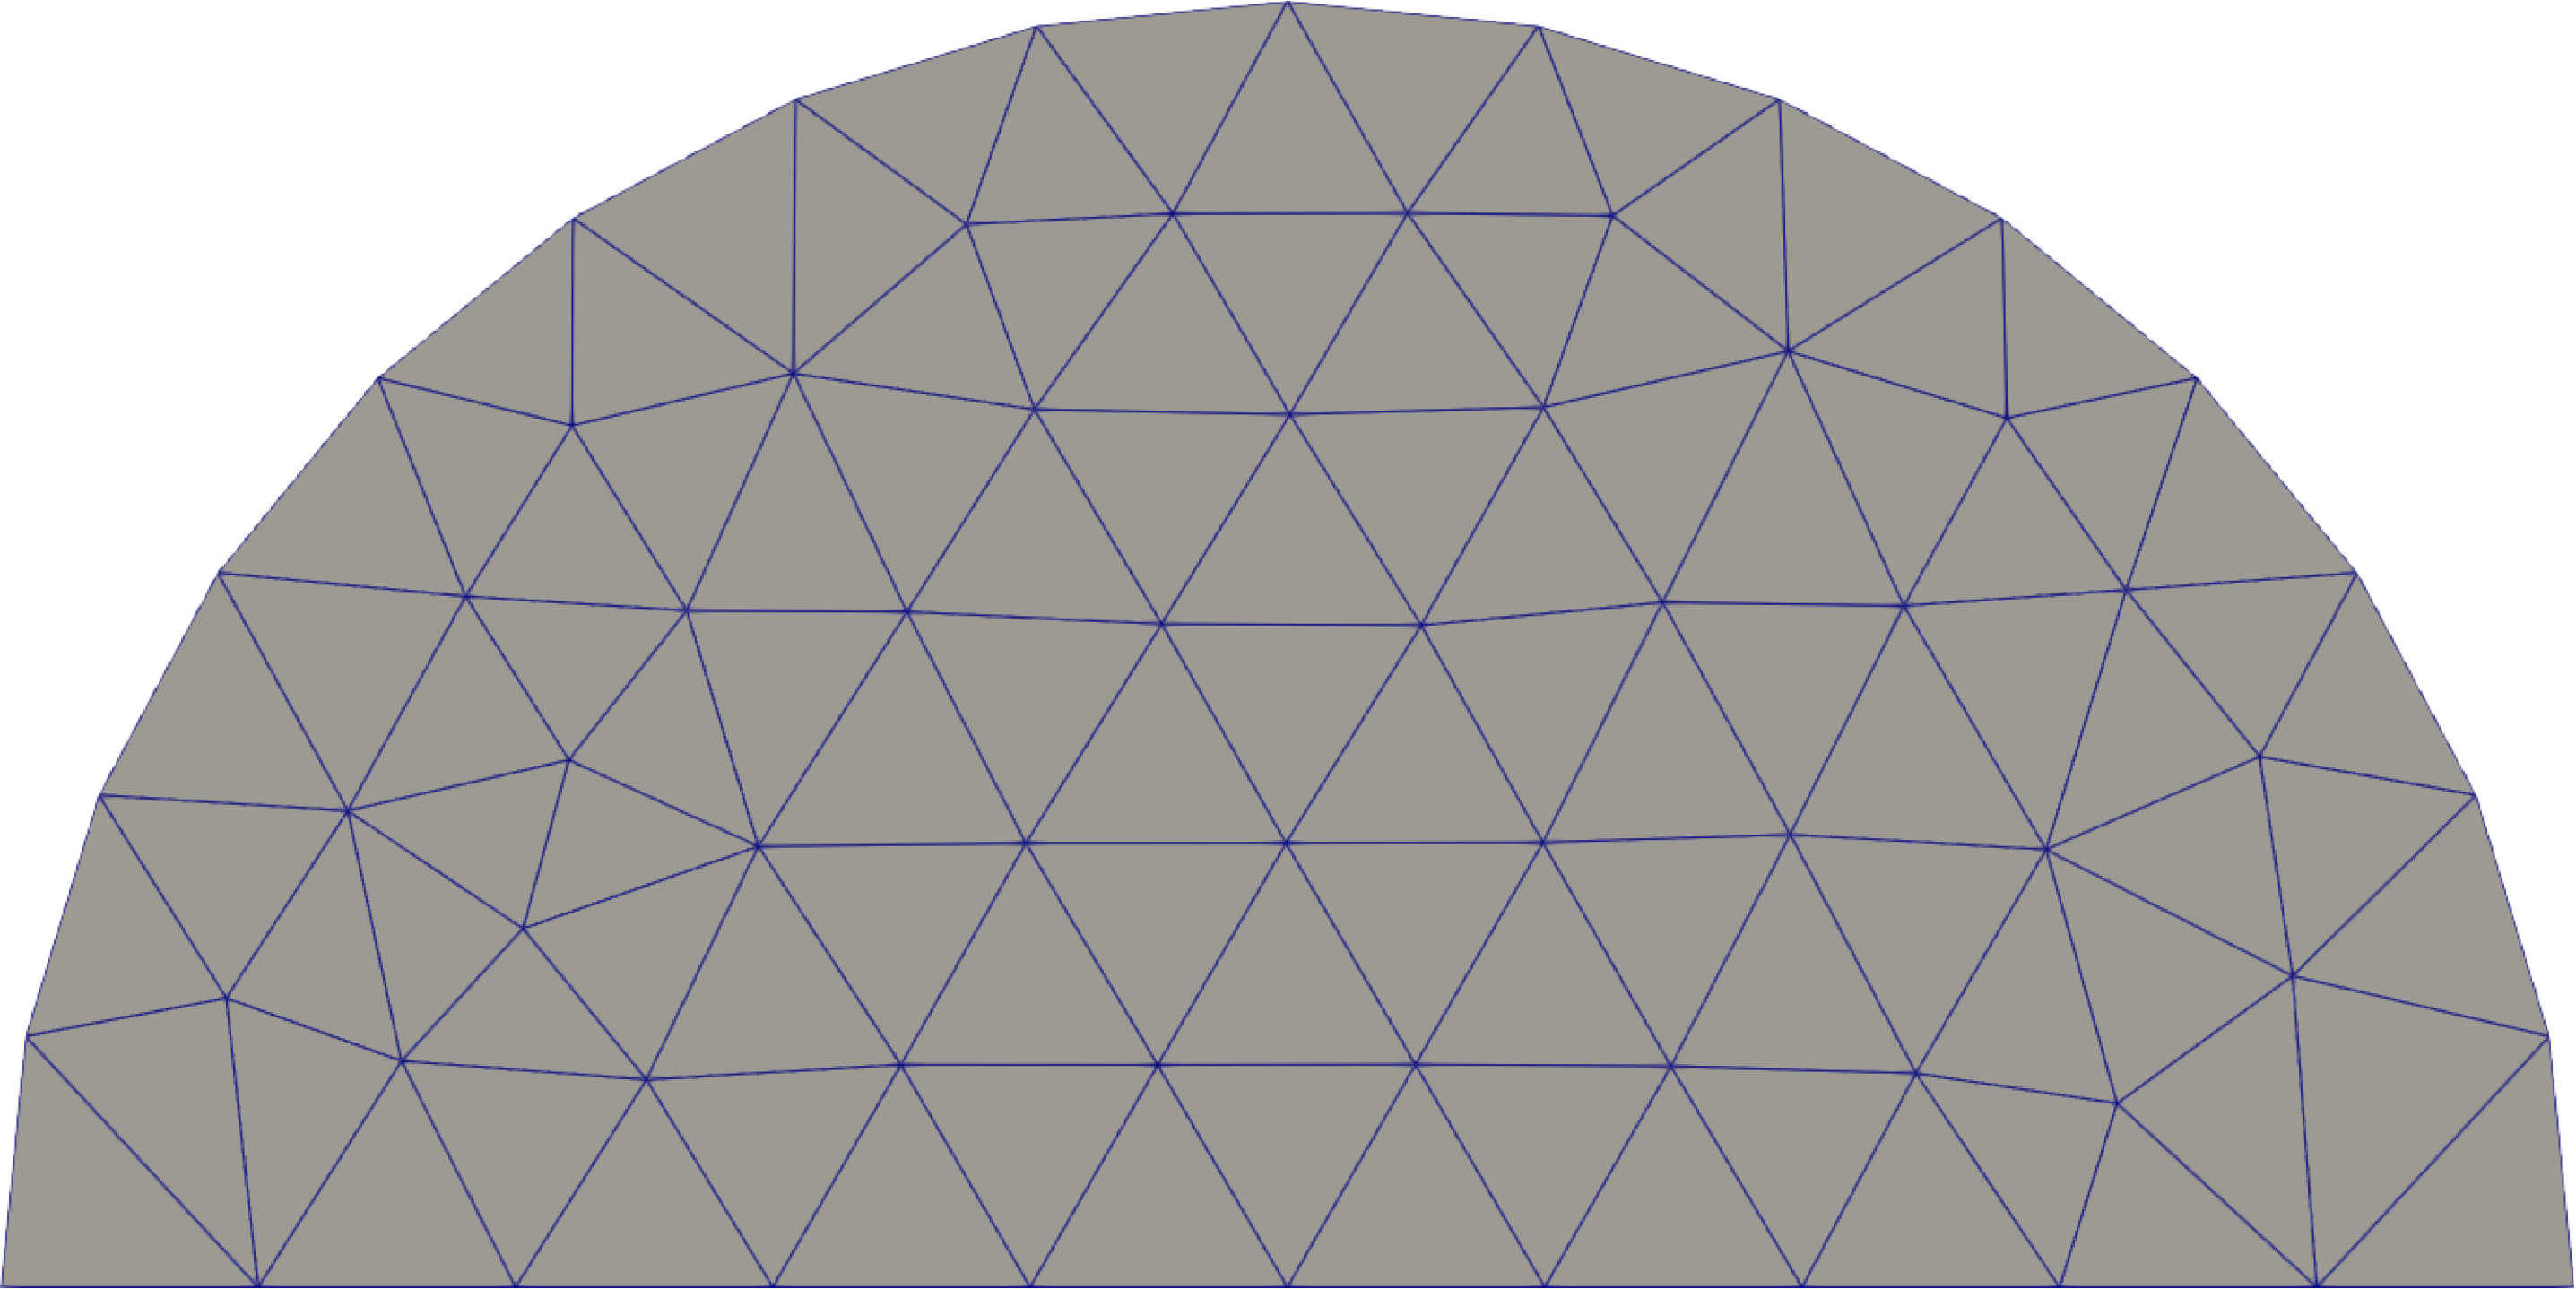
\includegraphics[width=\textwidth]{images/non_hermite_mesh_tri.pdf}
    \caption{Maillage triangulaire.}
    \label{fig:mail_tri_vs_mail_quad_1}
\end{subfigure}
\\[0.5cm]
\begin{subfigure}{0.6\textwidth}
    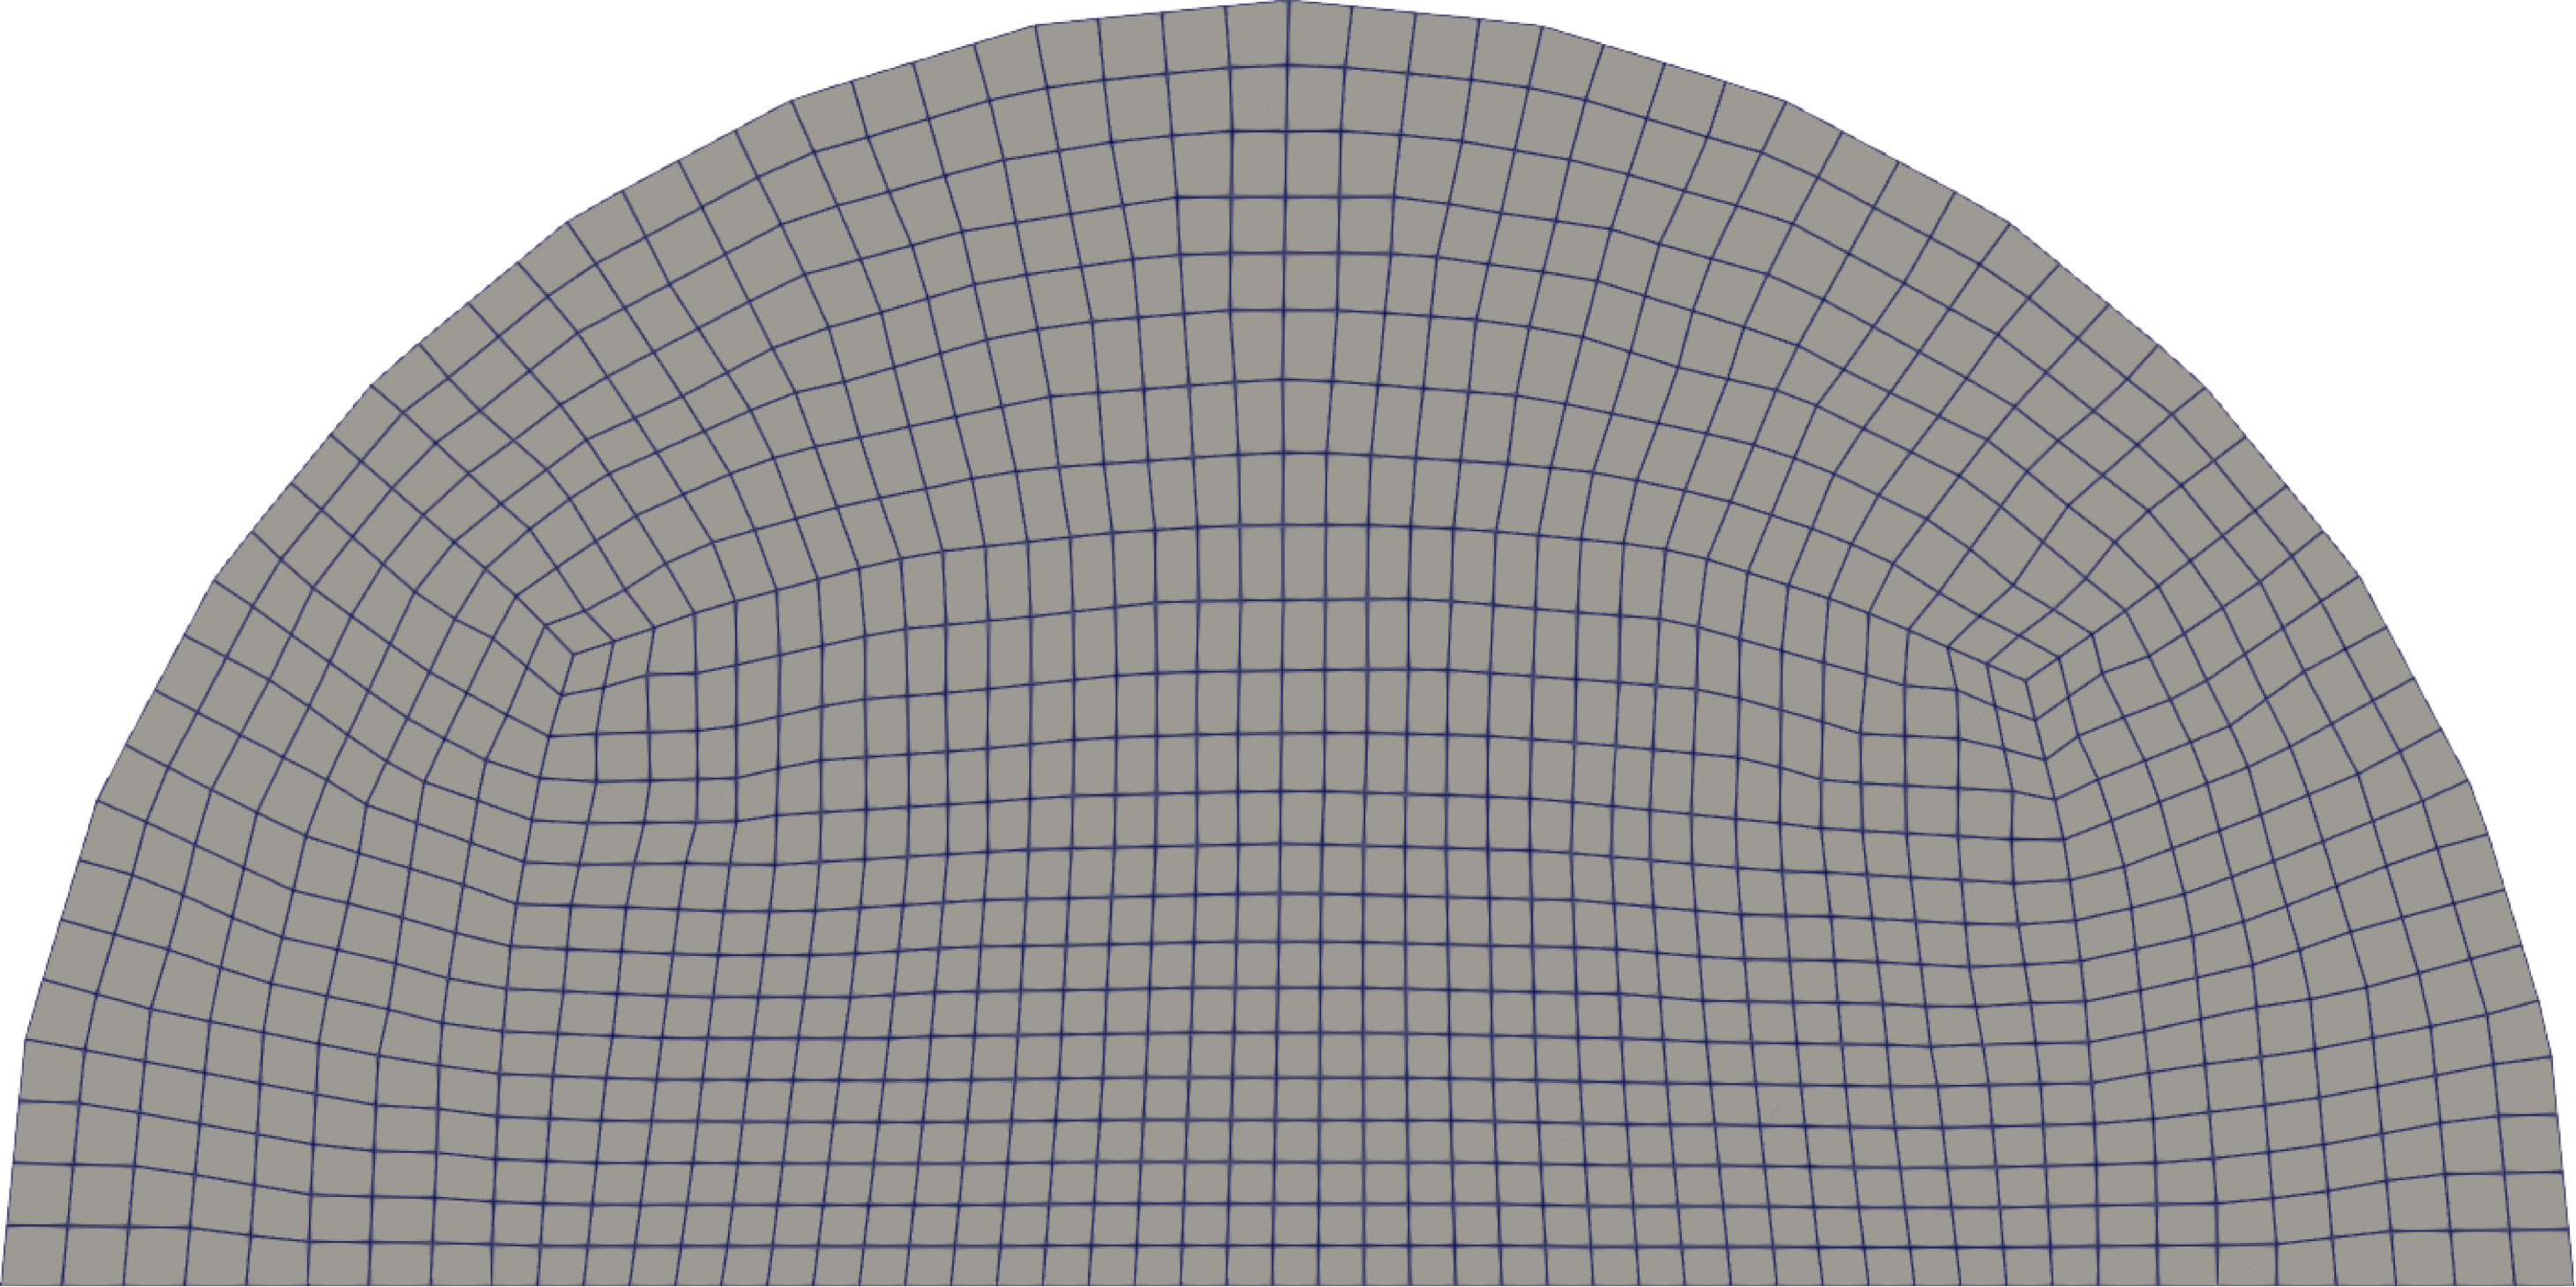
\includegraphics[width=\textwidth]{images/non_hermite_quad.pdf}
    \caption{Maillage quadrilatéral.}
    \label{fig:mail_tri_vs_mail_quad_2}
\end{subfigure}
\caption{Illustration d'un maillage quadrilatéral plus fin que le maillage triangulaire sous-jacent.}
\label{fig:mail_tri_vs_mail_quad}
\end{figure}
En utilisant une interpolation d'hermitte, on peut ainsi construire une reconstitution de régularité $\mathcal{C}^1$, $\partial\widetilde{\Omega_h}$ de $\partial\Omega_h$. Plus concrètement, soit $a$ et $b$ deux sommets de $\Omega_h$. L'arête $ab$ est remplacé par le polynôme $P$ défini pour tout $p\in ab$ par:
\[P(p) = q_a(p)P_a(p)+q_b(p)P_b(p),\]
où la fonction $q_x$, $x\in\{a, b\}$ est donné pour tout $p\in ab$ par:
\[q_x(p) = \prod_{y\in\{a,b\}, y\neq x} \left(\frac{p - y}{x - y}\right)^2,\]
et la fonction $P_x$, $x\in\{a, b\}$ est donné pour tout $p\in ab$ par:
\[P_x(p) = x + (p - x) \left(\mathcal{N}(x) - q_x'(x)x\right),\]
avec
\[q_x(x)=1,\quad\quad
q_x'(x)=\sum_{y\in\{a,b\}, y\neq x}\frac{2}{x - y},\quad\quad
\forall j \neq i \quad q_x'(y) = q_x(y) = 0.
\]
et $\mathcal{N}(x)$ est la normale sortante en $x$ définit par l'équation \eqref{eqn:n_reconstruit}.\\\\
Nous illustrons sur la figure \ref{fig:hermite} la Reconstitution d'une arête donné par ces deux sommets ainsi que les normales en ces sommets.


\begin{figure}[!h]
\centering
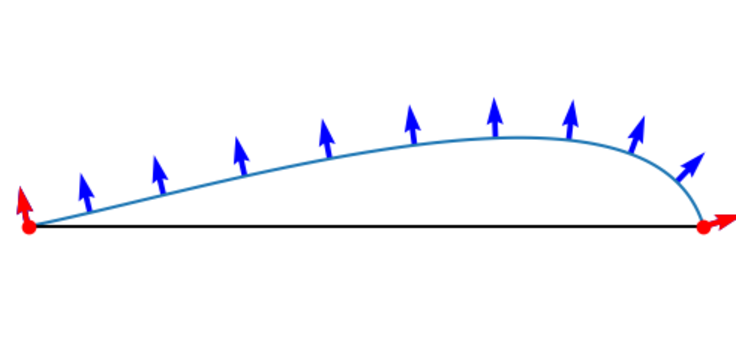
\includegraphics[scale=0.55]{images/hermite.pdf}
\caption{Illustration de la reconstitution d'une arête de bord par le molynôme d'Hermite.}
\label{fig:hermite}
\end{figure}

